%%%%%%%%%%%%%%%%%%%%%%%%%%%%%%%%%%%%%%%%%%%
%%% DOCUMENT PREAMBLE %%%
%This template was adapted from a template by Roza Aceska.
\documentclass[12pt]{report}
\usepackage[english]{babel}
%\usepackage{natbib}
\usepackage{url}
\usepackage[utf8x]{inputenc}
\usepackage{amsmath}
\usepackage{graphicx}
\usepackage{parskip}
\usepackage{fancyhdr}
\usepackage{vmargin}
\usepackage{caption}
\usepackage{subcaption}
\setmarginsrb{3 cm}{2.5 cm}{3 cm}{2.5 cm}{1 cm}{1.5 cm}{1 cm}{1.5 cm}

\title{Report Assignment Part 1}								
% Title
\author{}						
% Author
\date{}
% Date

\makeatletter
\let\thetitle\@title
\let\theauthor\@author
\let\thedate\@date
\makeatother

\pagestyle{fancy}
\fancyhf{}
\rhead{\theauthor}
\lhead{\thetitle}
\cfoot{\thepage}
%%%%%%%%%%%%%%%%%%%%%%%%%%%%%%%%%%%%%%%%%%%%
\begin{document}

%%%%%%%%%%%%%%%%%%%%%%%%%%%%%%%%%%%%%%%%%%%%%%%%%%%%%%%%%%%%%%%%%%%%%%%%%%%%%%%%%%%%%%%%%

\begin{titlepage}
	\centering
    \vspace*{0.5 cm}
  \begin{center}    \textsc{\Large   Adavanced Process Mining SS20}\\[2.0 cm]	\end{center}
	\rule{\linewidth}{0.2 mm} \\[0.4 cm]
	{ \huge \bfseries \thetitle}\\
	\rule{\linewidth}{0.2 mm} \\[1.5 cm]
	
  \begin{minipage}{0.48\textwidth}
    \begin{flushleft} \large
      \emph{Submitted To:}\\
      Tobias Brockhoff\\
      Lisa Mannel\\
      Sebastiaan J. van Zelst MSc PhD\\
    \end{flushleft}
  \end{minipage}~
  \begin{minipage}{0.48\textwidth}
    \begin{flushright} \large
			\emph{Submitted By:} \\
      Student 1 (Matr. Number) \\
      Bruno Machado Pacheco (403532)  \\
      Tom-Hendrik Hülsmann (355773)
		\end{flushright}
	\end{minipage}\\[2 cm]
	
\end{titlepage}

%%%%%%%%%%%%%%%%%%%%%%%%%%%%%%%%%%%%%%%%%%%%%%%%%%%%%%%%%%%%%%%%%%%%%%%%%%%%%%%%%%%%%%%%%

\renewcommand{\thesection}{\arabic{section}}

\section{Q1. Inductive Miner}

As a first step into discovering the model for the event log, a short exploration was carried before the application of the algorithm. This to familiarize ourselves with the provided data. Besides a visualization of the dataset, a report was automatically generated with a data-centered description. Also, a brief analysis on the cardinality of the relation between traces and the \emph{Patient} column, which was found to be 1:1. Lastly, some random traces were visualized.

\paragraph{a)} 

Overall, we can estimate that the patients situation is assessed through an initial exam and, if necessary, 4 different treatments can be applied. In the process tree generated, visible in Figure \ref{fig:figures-q1_a_tree-pdf}, it is possible to identify the exclusive decision made between the discharge of the initial exam and the isolation inform, but the model fails to identify the relation between this decision and the application of the treatments, that certainly must occur only in infected patients.

\begin{figure}[h]
    \centering
    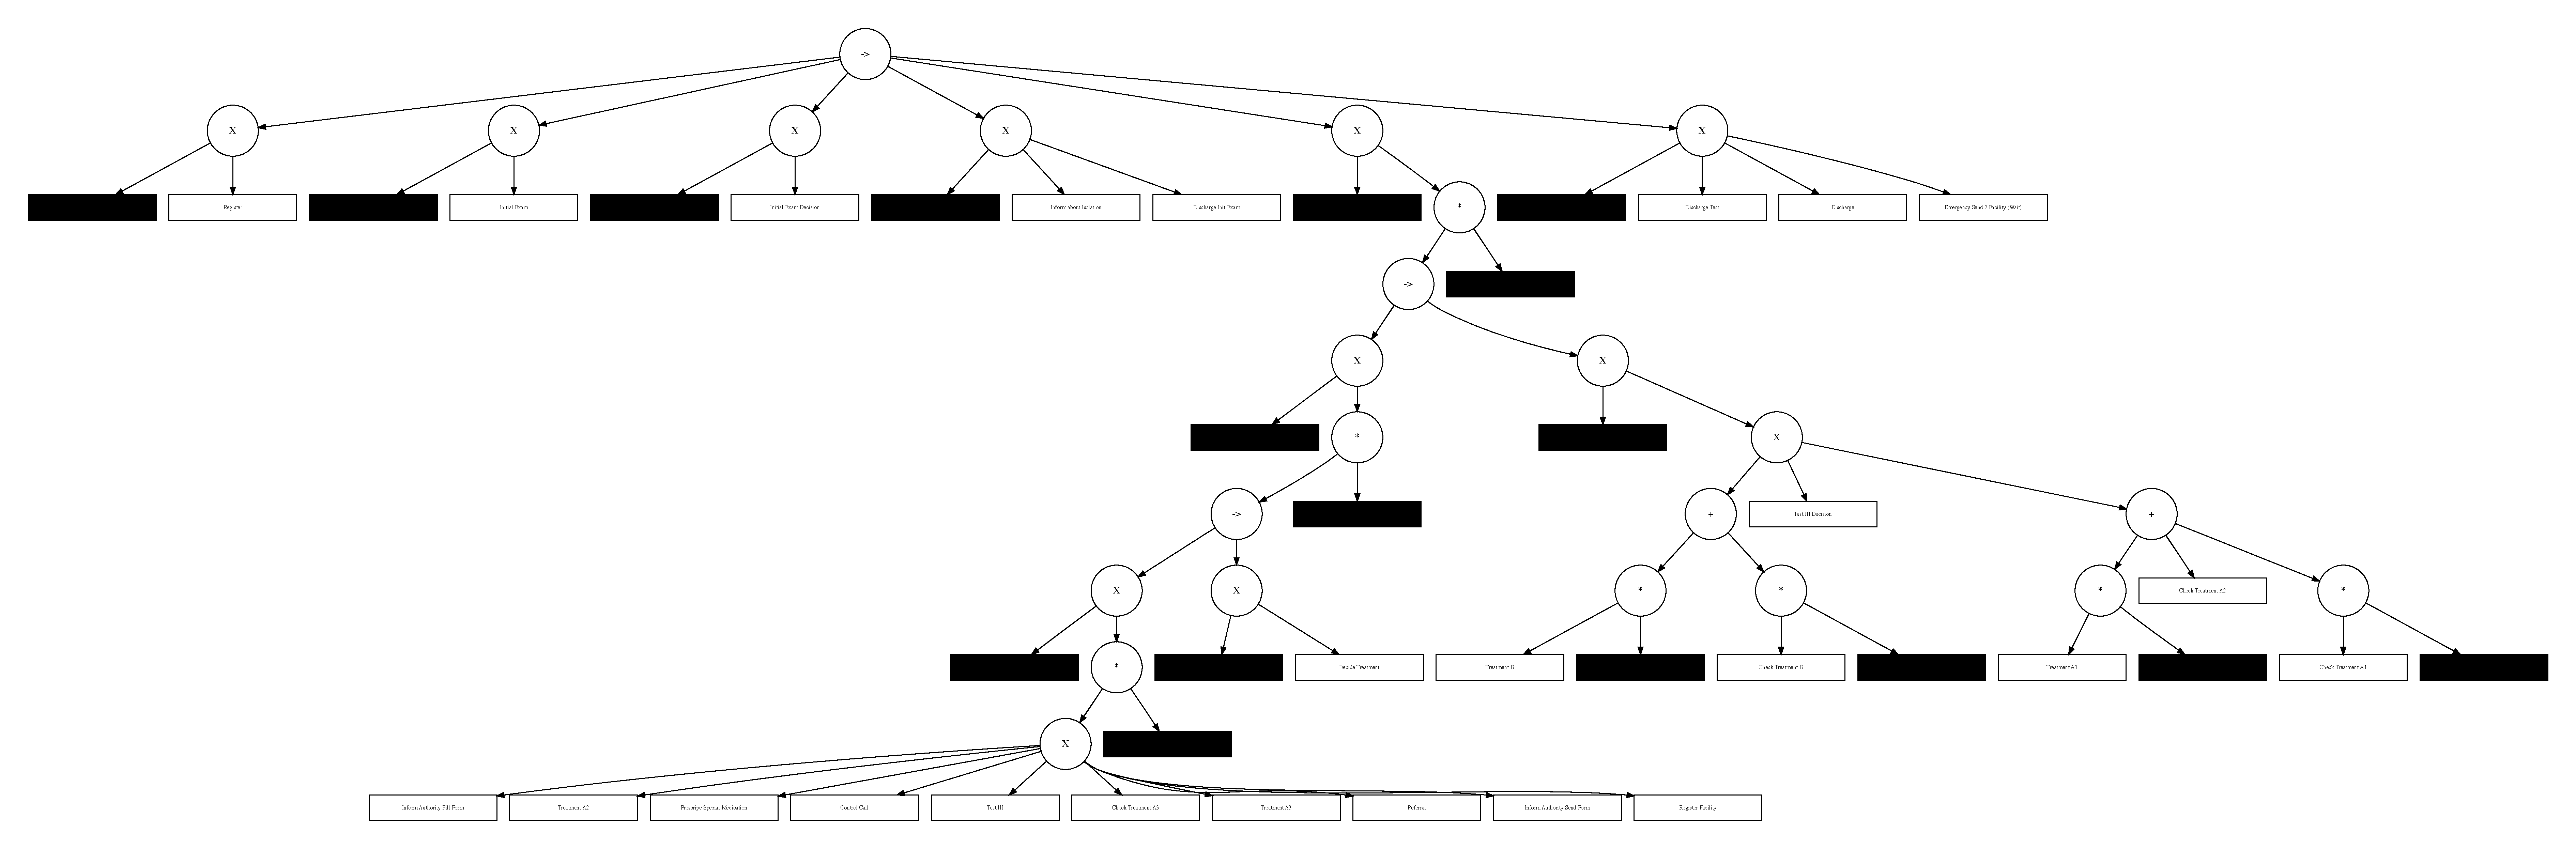
\includegraphics[width=\textwidth]{figures/q1_a_tree.pdf}
    \caption{Process Tree generated by the Inductive Miner}
    \label{fig:figures-q1_a_tree-pdf}
\end{figure}

The treatments are applied multiple times alternating with the respective \emph{Check} activity. Unfortunately, the models are not too helpful in describing the choice of the treatments nor the dynamics of the execution of the remaining activities after the isolation inform. The exceptions are the ending activities, which tells us that the patients can either be discharged or sent to emergency care.

We notice the Inductive Miner guarantee for perfect fitness in the generated model through the presence of several silent transitions, an known outcome of the algorithm mainly present in the outcome of noisy event logs. Another characteristic of the IM is its inability to capture non-local dependencies, as it is shown more obviously, as already mentioned, by the lack of relation between the result of the initial exam and the applications' of the treatments. A more subtle consequence of this characteristic is the inability to constrain the `Check Treatment *` activities to follow, not necessarily directly, the respective treatment activity.

Regarding its precision, we notice there are several characteristics of the process that the model is unable to represent, using underfitting approaches instead. Besides the two mentioned just above, we point out the flower structure in the lowest level of the process tree and the more abstract flower pattern in the second-last exclusive choice operator of the second level. Therefore, we can say that the generated model is perfectly fit to the log, as expected, but not very precise.

The two main reasons identified for the lack of preciseness are the excess of silent transitions and the use of generalist structures (flower pattern). We can estimate that the first may be caused by noise in the data, which is usual. The second can be caused by a limitation of the algorithm, that is unable to deal with non-local dependencies.

\paragraph{b)} 

After distinguishing the two instances of the \emph{Control Call} activity in the event log, the Inductive Miner was again applied and the resulting model can be seen in Figure \ref{fig:figures-q1_b_tree-pdf} below.

\begin{figure}[h]
    \centering
    
\includegraphics[width=\textwidth]{figures/q1_b_tree.pdf}
    \caption{Process Tree after \emph{Control Call} splitting}
    \label{fig:figures-q1_b_tree-pdf}
\end{figure}

We can see that not only the `Control Call` activity was removed from the flower structure at the bottom, but also the `Test III` and `Test III Decision` were brought up to the first sequence operator, of course still within a exclusive-choice operator with a silent activity, due to the noise on the data.

Still, now it is possible to extend our assumptions about the process. After the initial exam proceedings, several control calls can be performed and they are followed by the \emph{Test III}, which defines if the patient will need treatment.

\paragraph{c)} 

After filtering the DFG we can already notice an improvement. The absence of many of the edges in the original DFG made the filtered one much more linear and readable. Still, we can also notice the structure of the activities related to the A treatments is not properly captured. The two DFGs can be seen in Figure \ref{fig:dfg-filtering}.

\begin{figure}[h]
    \centering
    \begin{subfigure}[b]{0.4\textwidth}
	\centering
	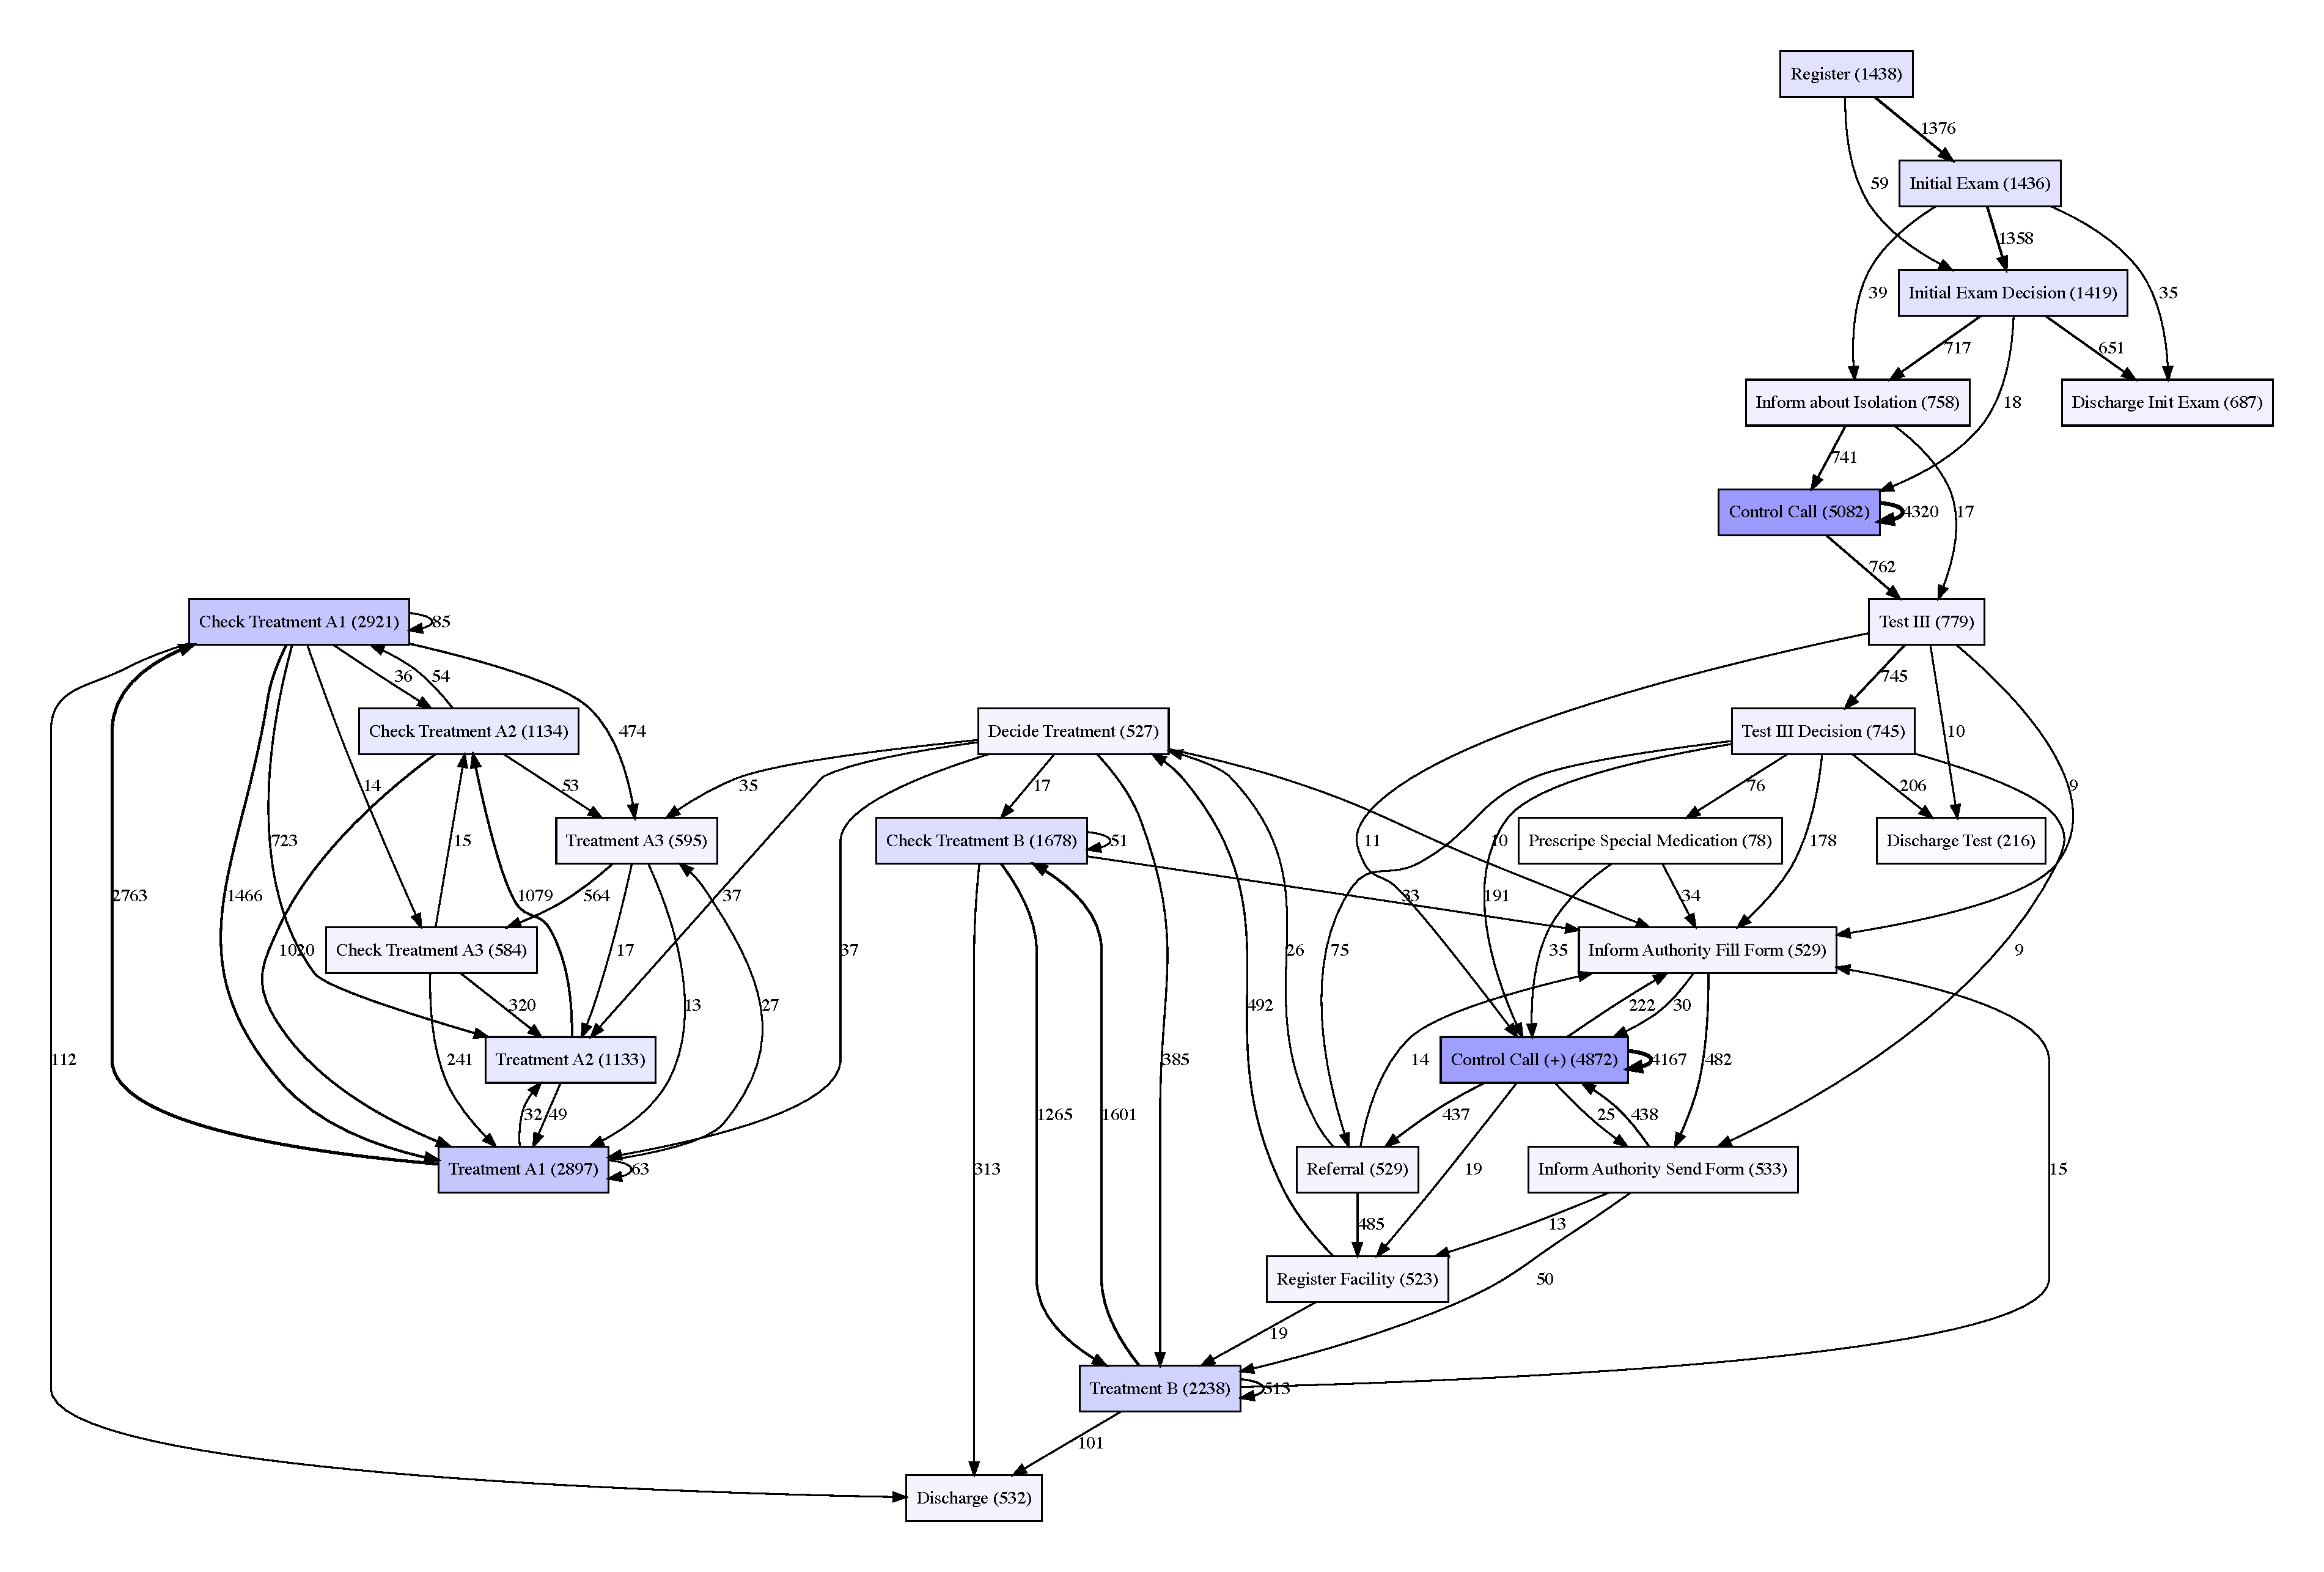
\includegraphics[width=\textwidth]{figures/q1_c_dfg_renaming.pdf}
	\caption{DFG generated after context-sensitive renaming}
	\label{fig:subfigures-q1_c_dfg_renaming-pdf}
    \end{subfigure}
    \hfill
    \begin{subfigure}[b]{0.4\textwidth}
	\centering
	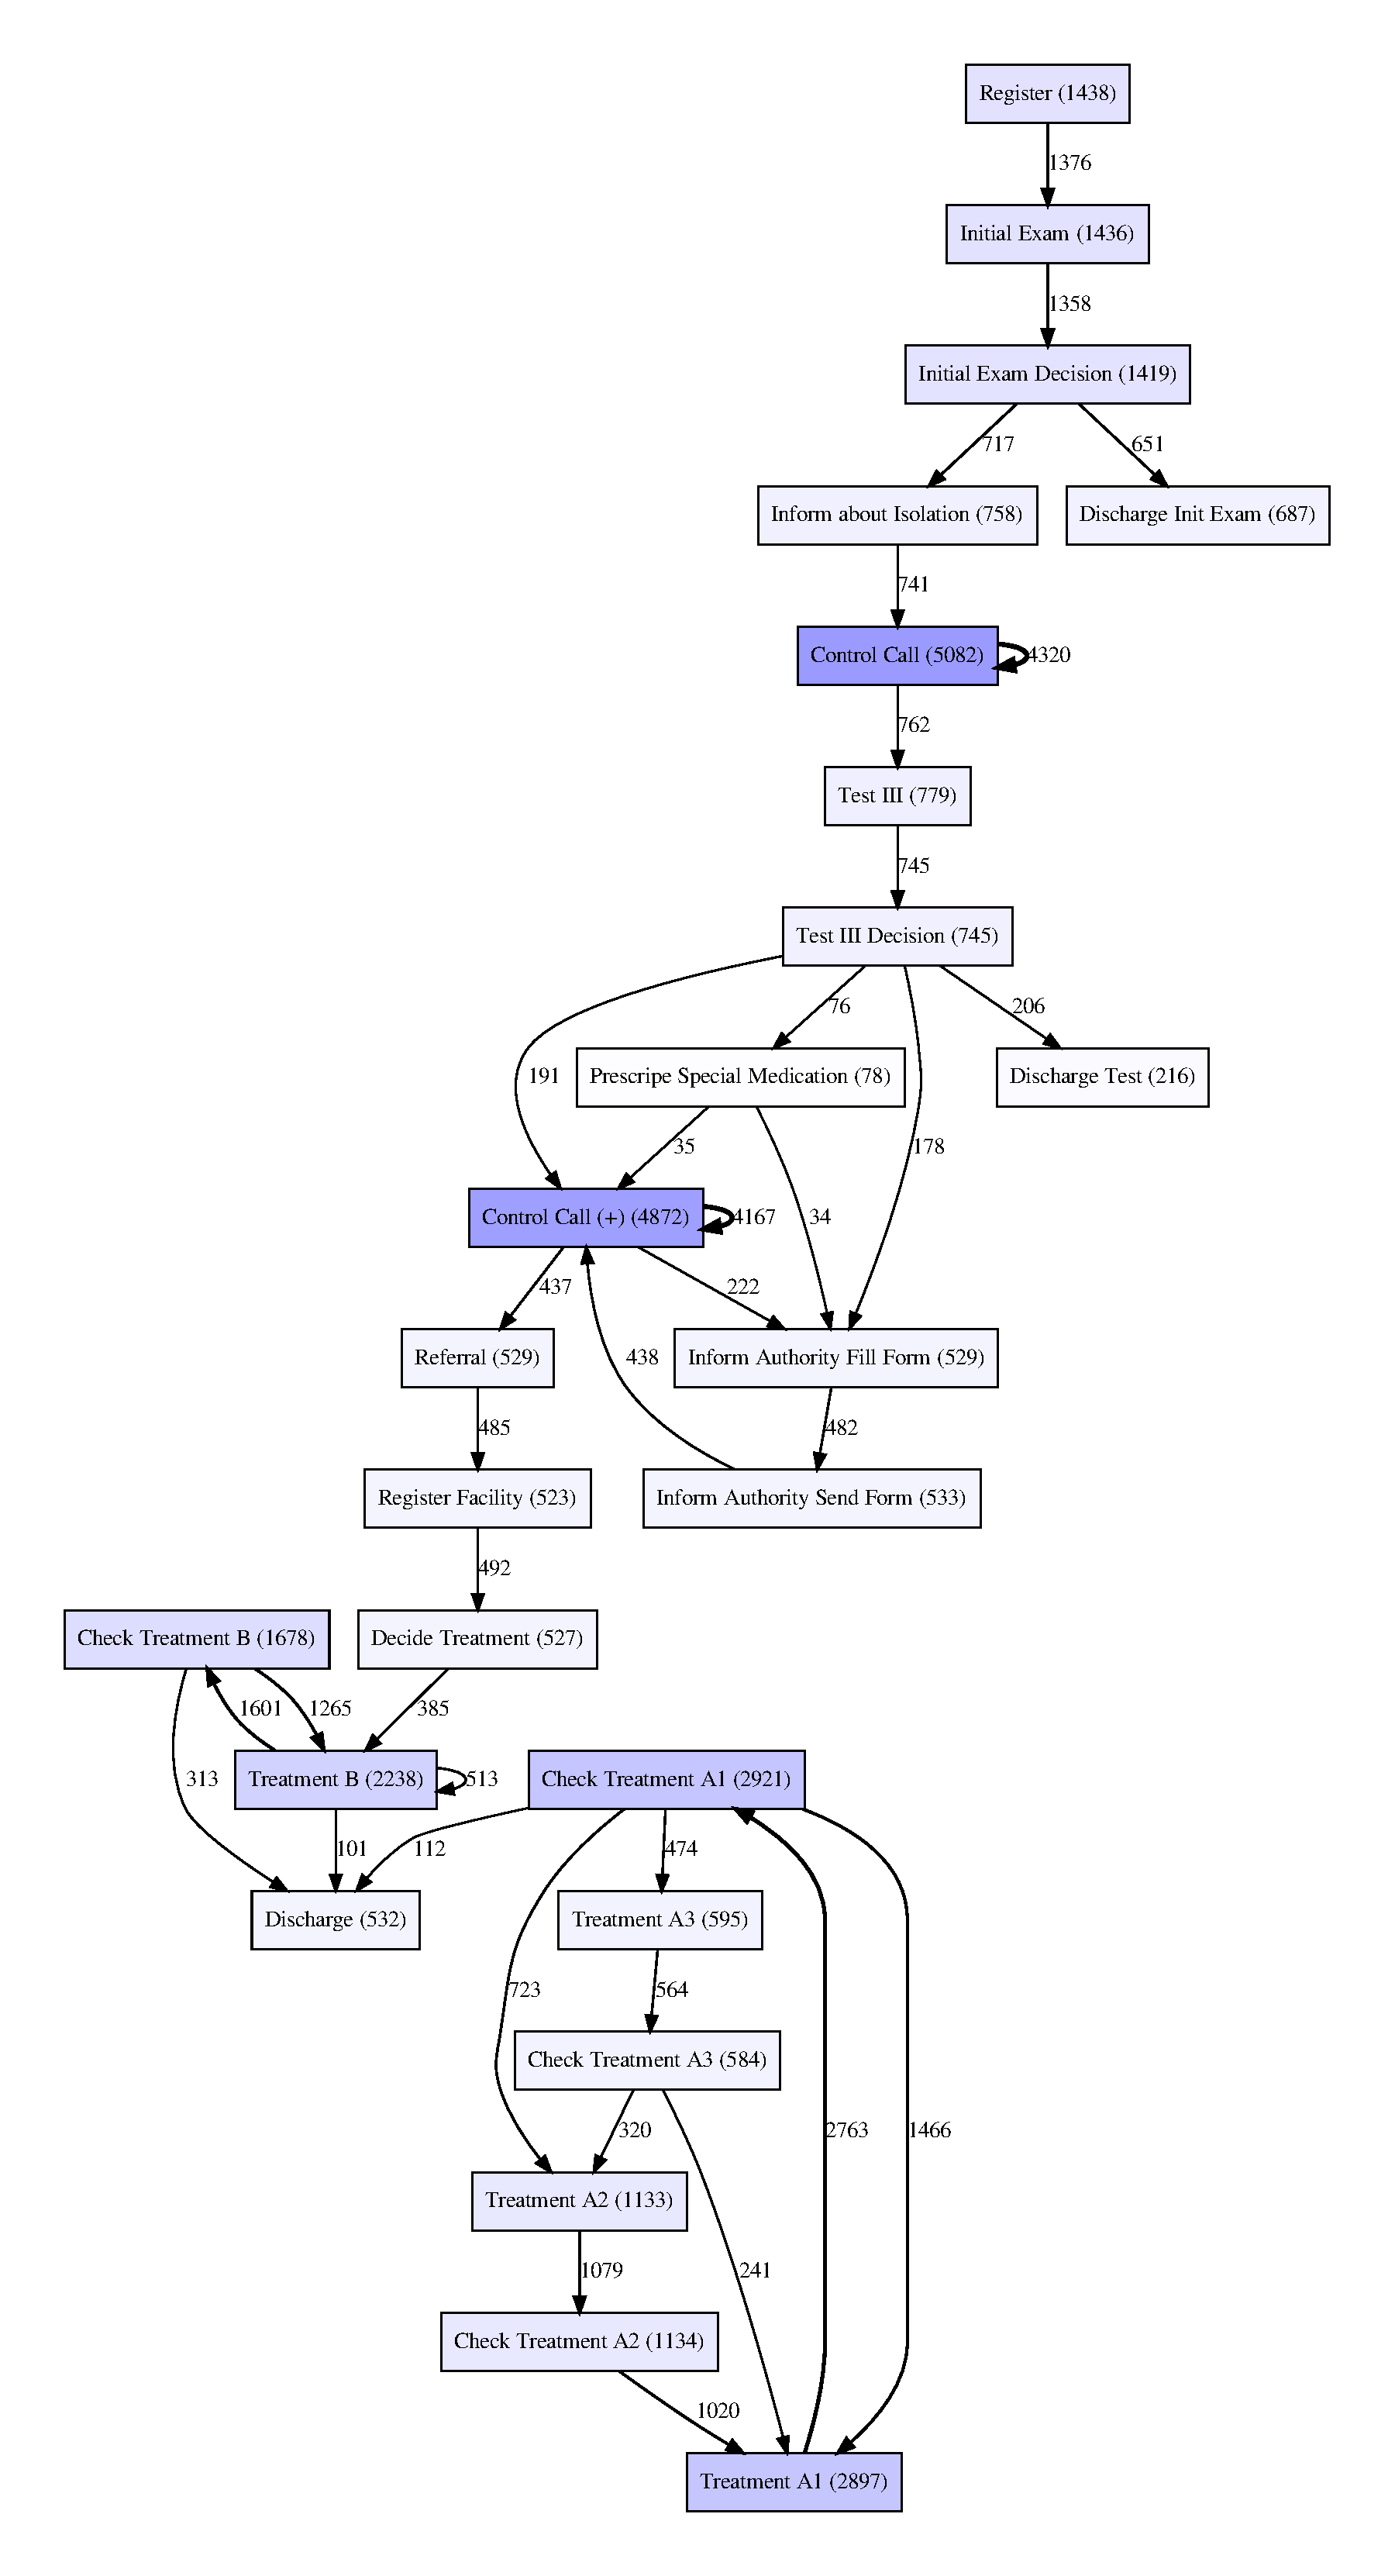
\includegraphics[width=\textwidth]{figures/q1_c_dfg_filtered.pdf}
	\caption{Filtered DFG}
	\label{fig:subfigures-q1_c_dfg_filtered-pdf}
    \end{subfigure}
    \hfill
    \caption{DFG filtering}
    \label{fig:dfg-filtering}
\end{figure}

Upon the filtered DFG, the IM algorithm was run once again and the resulting process tree can be seen in Figure \ref{fig:figures-q1_c_filt_tree-pdf}. The new model generated is much closer to the expected from the superficial analysis of the traces. The noise removed comes mostly from skipped activities, that were not logged, as we can notice through the edges in the DFG that were removed.

Still, the structure of the activities related to the treatment A variants was not captured. One can notice in the bottom of the filtered DFG that the nodes related to these treatments are only connected to the remaining of the graph through the \emph{Discharge} activity, which is supposed to be one of the final activities. This implied in the loop operator right next to the \emph{Register} activity in the process tree and the subsequent silent activities. We estimate this problem was caused by the relative rarity (123 out of 1500) of traces in which these activities are performed, but since they are performed several times for each trace, the edges between these activities were not filtered.

\begin{figure}[h]
    \centering
    
\includegraphics[width=\textwidth]{figures/q1_c_filt_tree.pdf}
    \caption{Process tree generated by the IM application on the filtered DFG}
    \label{fig:figures-q1_c_filt_tree-pdf}
\end{figure}

\paragraph{d)} 

Based on the discussed in the previous, we identify two approaches for the problem with the activities related to the A treatments: the first would be to remove them from the log; the second would be to fine tune the filtering threshold so no to remove the edges from the DFG that relate these activities from the others.

Removing these activities we get the model seen in Figure \ref{fig:dfg-pt-no-A}. Even though we had a great improvement in the structures represented caused by the removal of the pending structure as discussed above. Still, the algorithm fails to understand the sequence structure that should have happened after the non-execution of the \emph{Discharge Init Exam} activity, therefore inserts several silent activities along the tree. Other than that, the operators around the \emph{Control Call} activity after the test are not precise as are not as well the operators that deal with the treatment B related activities. 

\begin{figure}[h]
    \centering
    \begin{subfigure}[b]{0.2\textwidth}
        \centering
	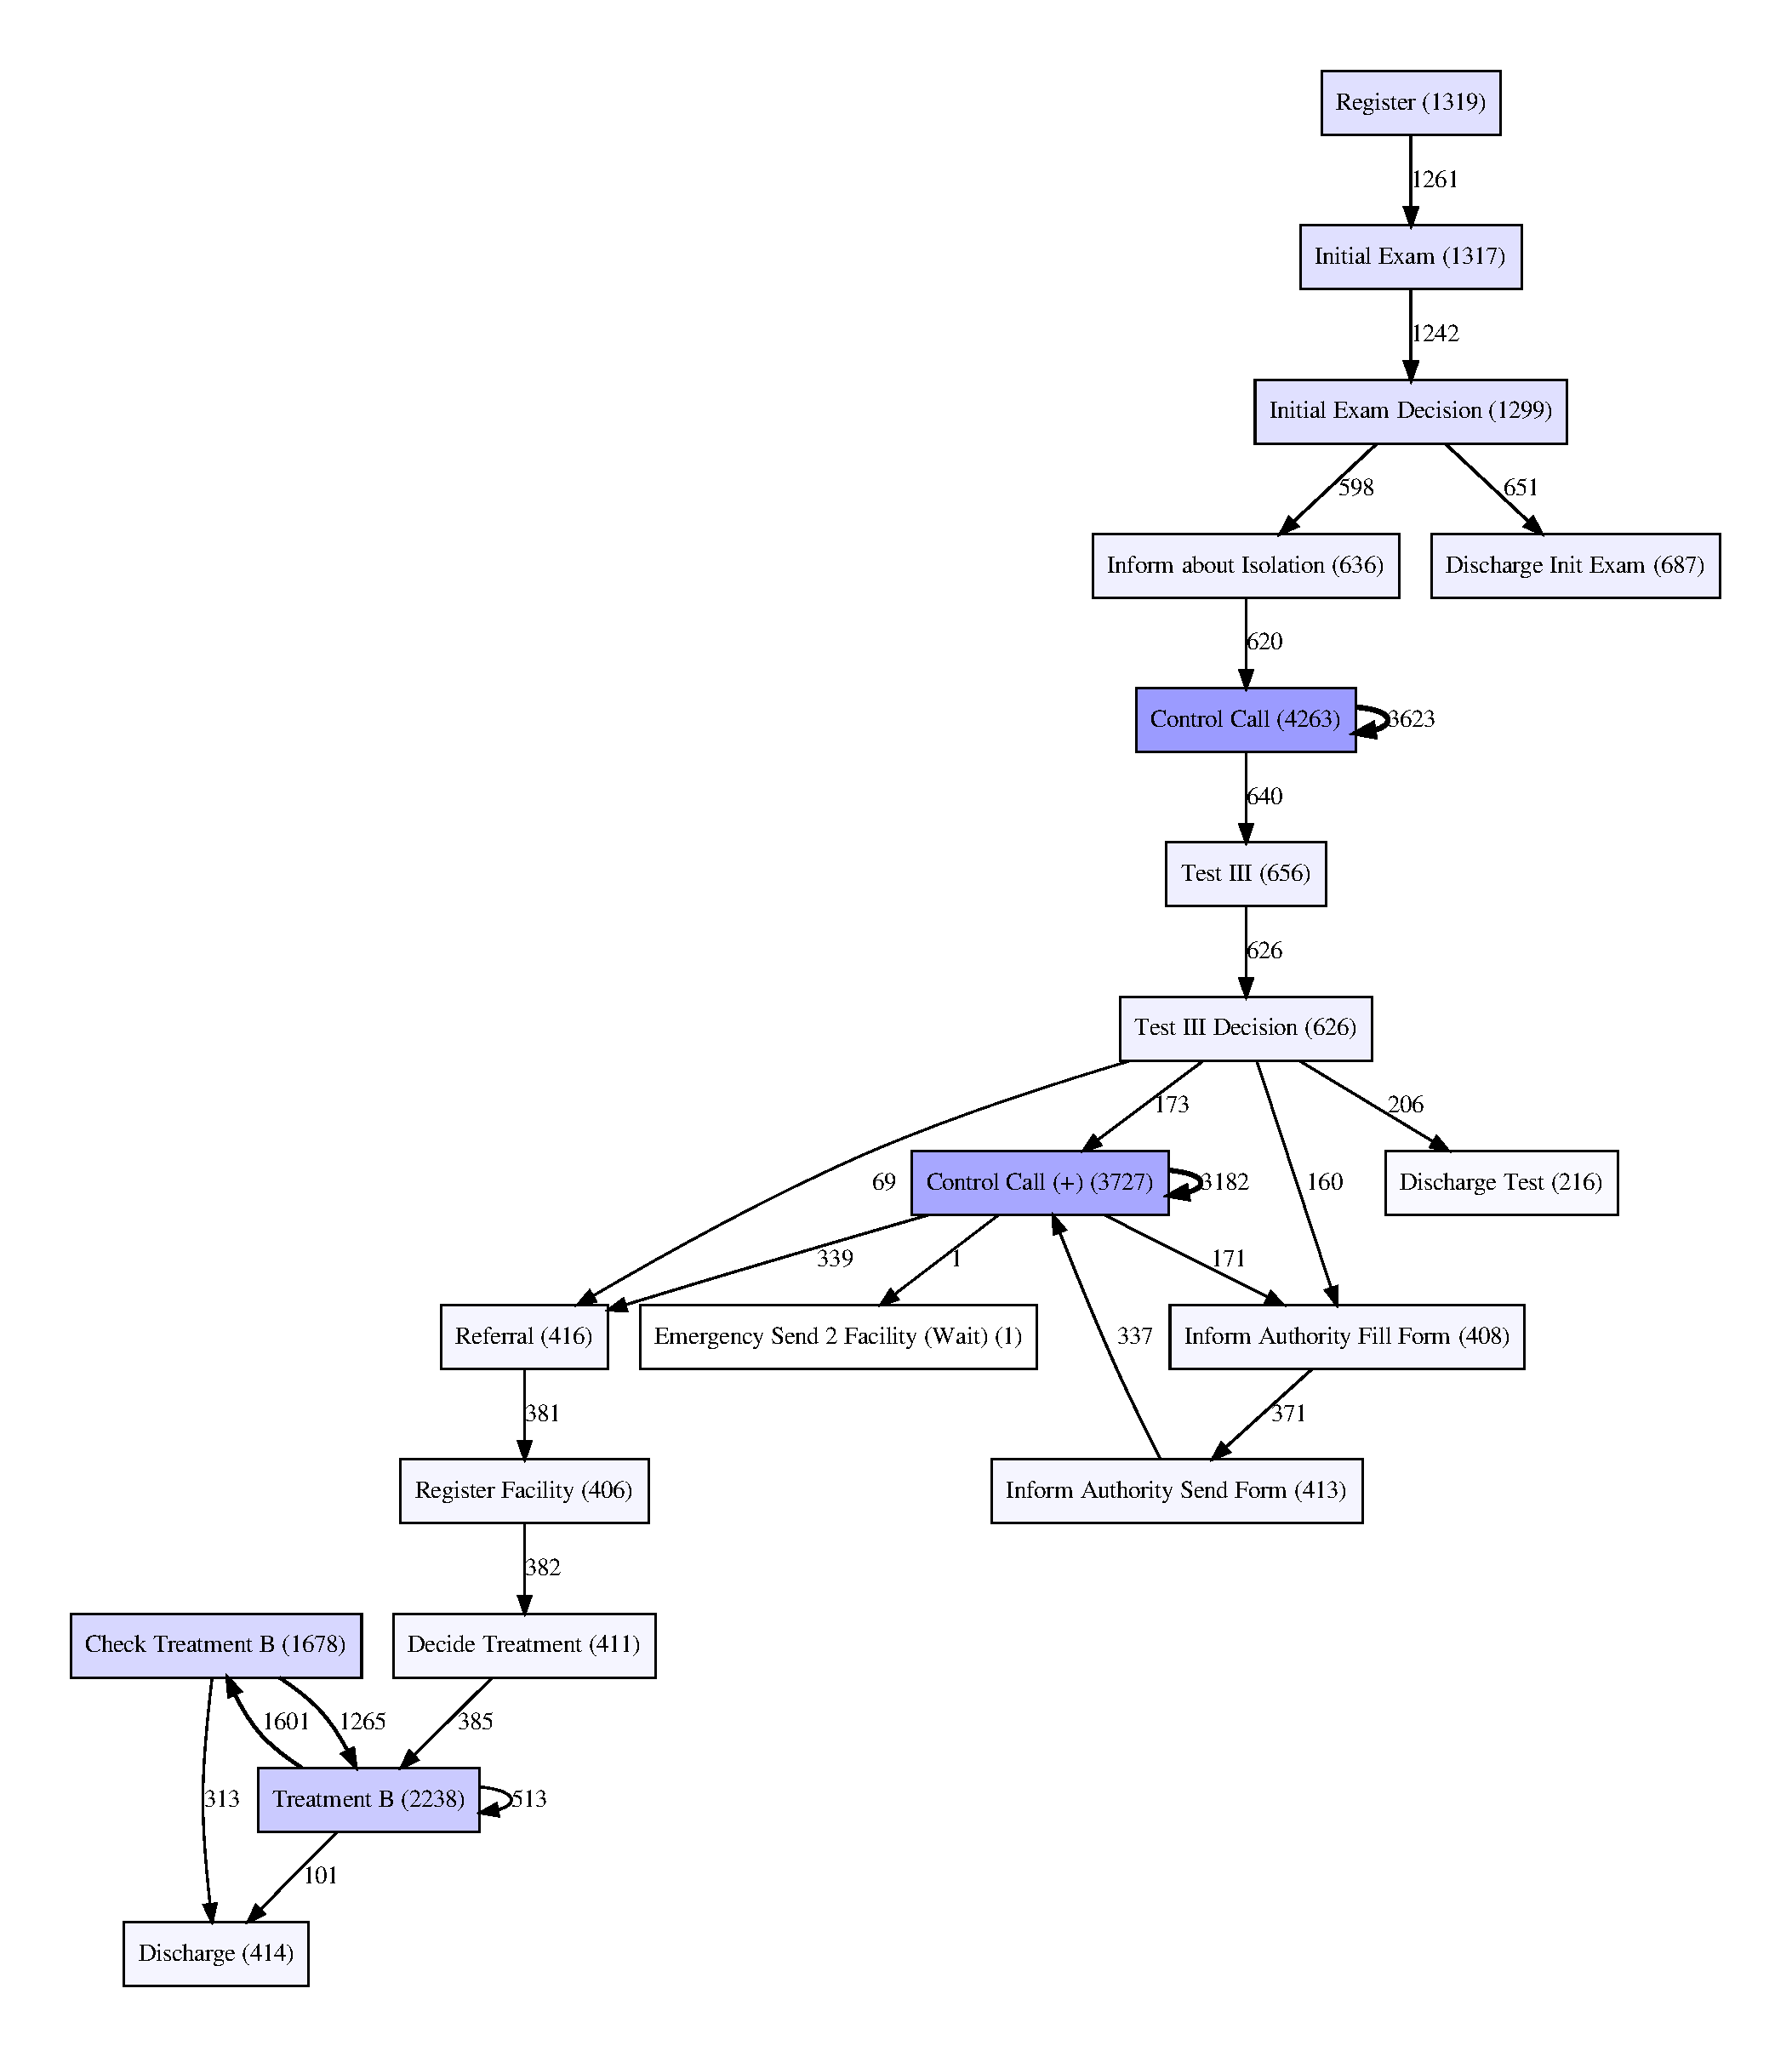
\includegraphics[width=\textwidth]{figures/q1_d_no_A.pdf}
        \caption{DFG}
        \label{fig:figures-q1_d_no_A-pdf}
    \end{subfigure}
    \hfill
    \begin{subfigure}[b]{0.7\textwidth}
        \centering
	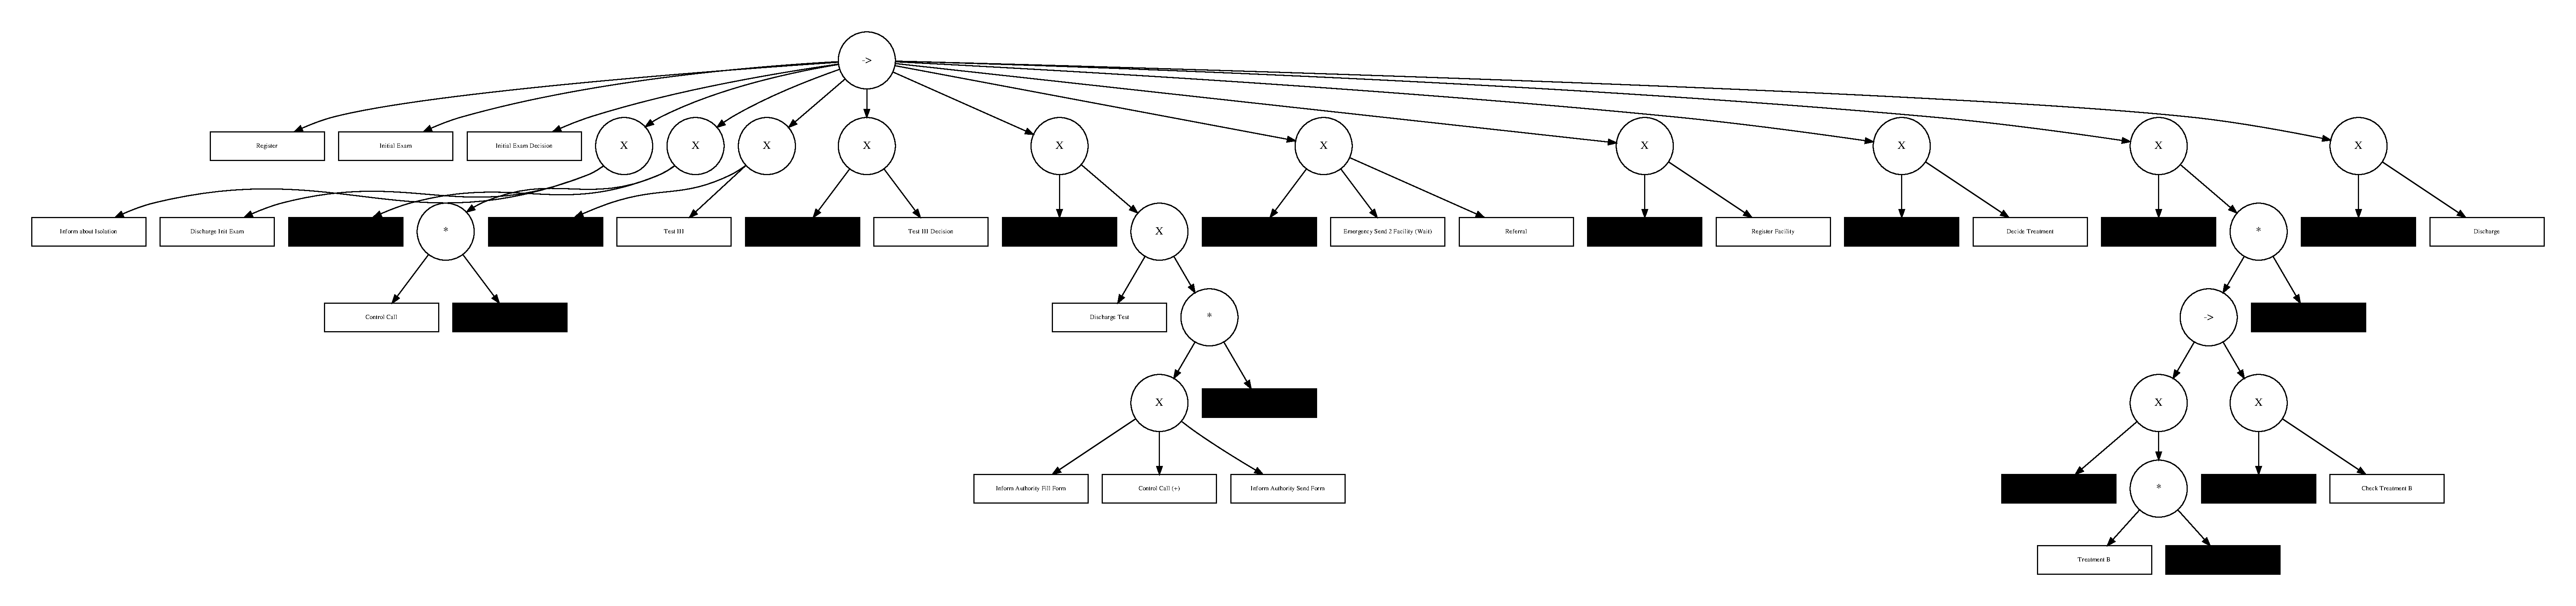
\includegraphics[width=\textwidth]{figures/q1_d_tree_no_A.pdf}
        \caption{Process Tree}
        \label{fig:figures-q1_d_tree_no_A-pdf}
    \end{subfigure}
    \hfill
    \caption{Model resulting after the filtering of the traces containing activities related to the A treatments}
    \label{fig:dfg-pt-no-A}
\end{figure}

A side effect of removing theses traces is that the \emph{Prescripe Special Medication} activity vanished, so we removed just the activities, keeping the traces, which had the precise effect of bringing the mentioned activity back to the model, as can be seen in Figure \ref{fig:dfg-pt-silent-A}.

\begin{figure}[h]
    \centering
    \begin{subfigure}[b]{0.2\textwidth}
        \centering
	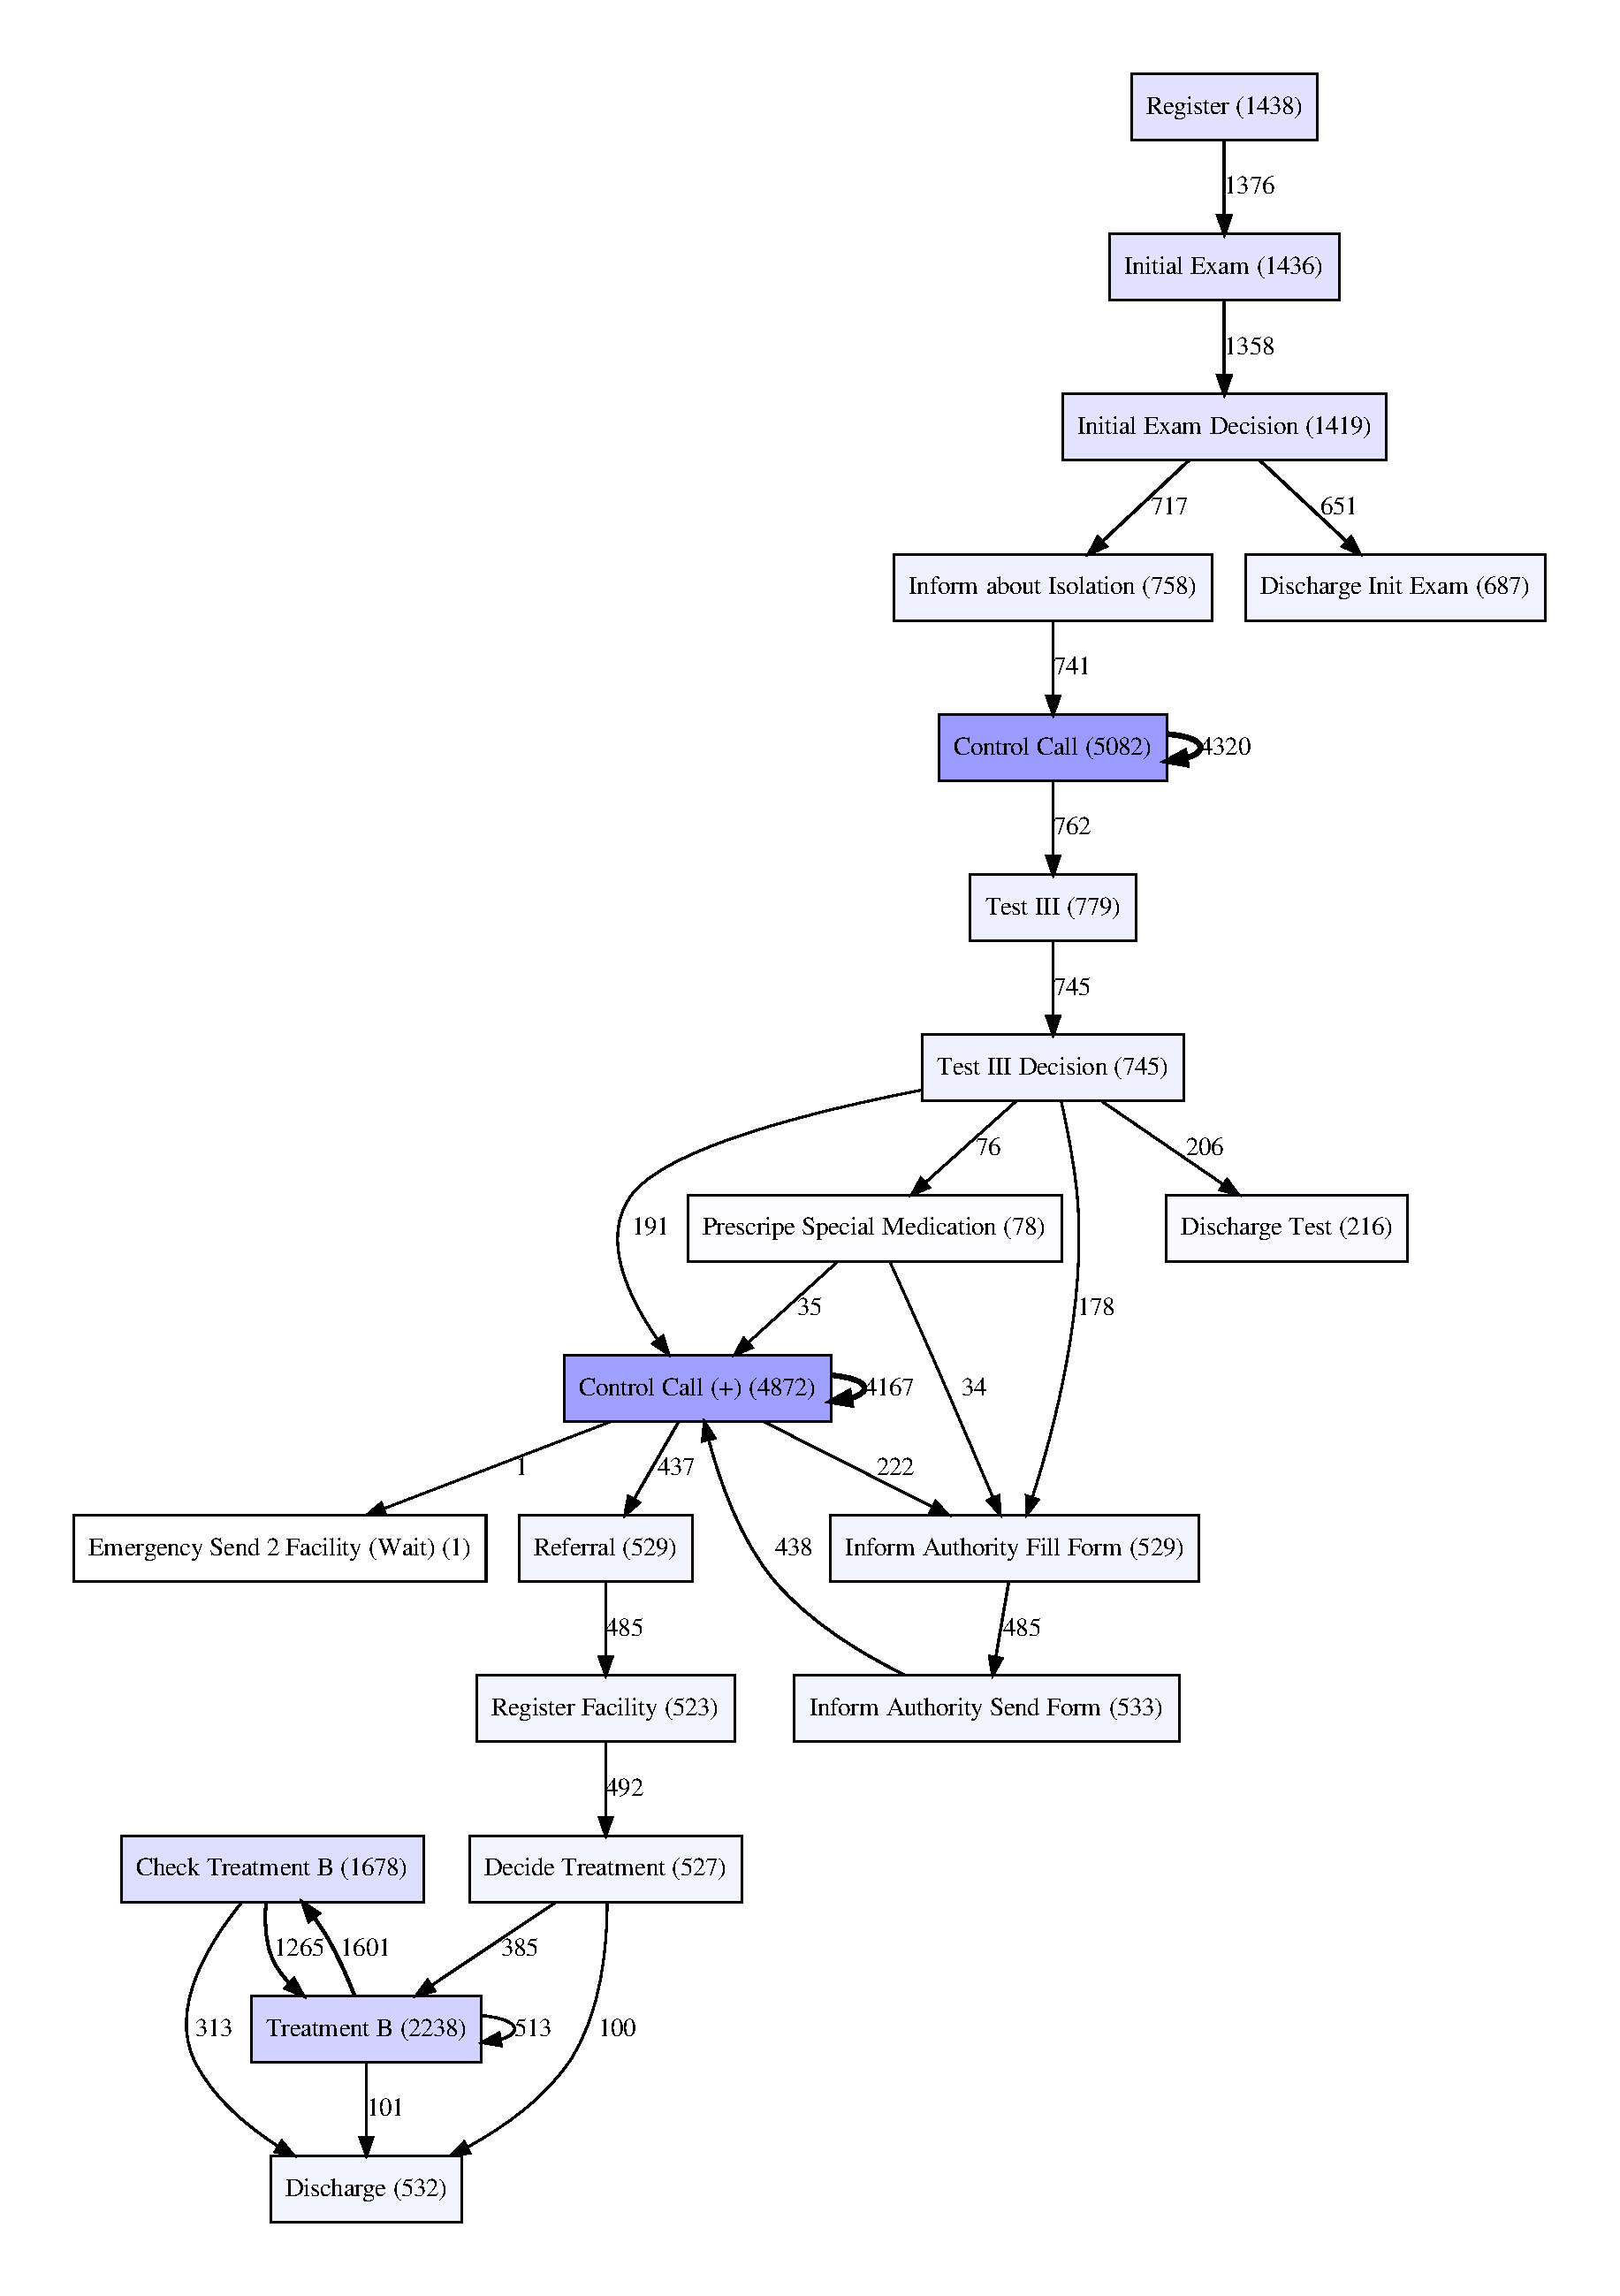
\includegraphics[width=\textwidth]{figures/q1_d_silent_A.pdf}
        \caption{DFG}
        \label{fig:figures-q1_d_silent_A-pdf}
    \end{subfigure}
    \hfill
    \begin{subfigure}[b]{0.7\textwidth}
        \centering
	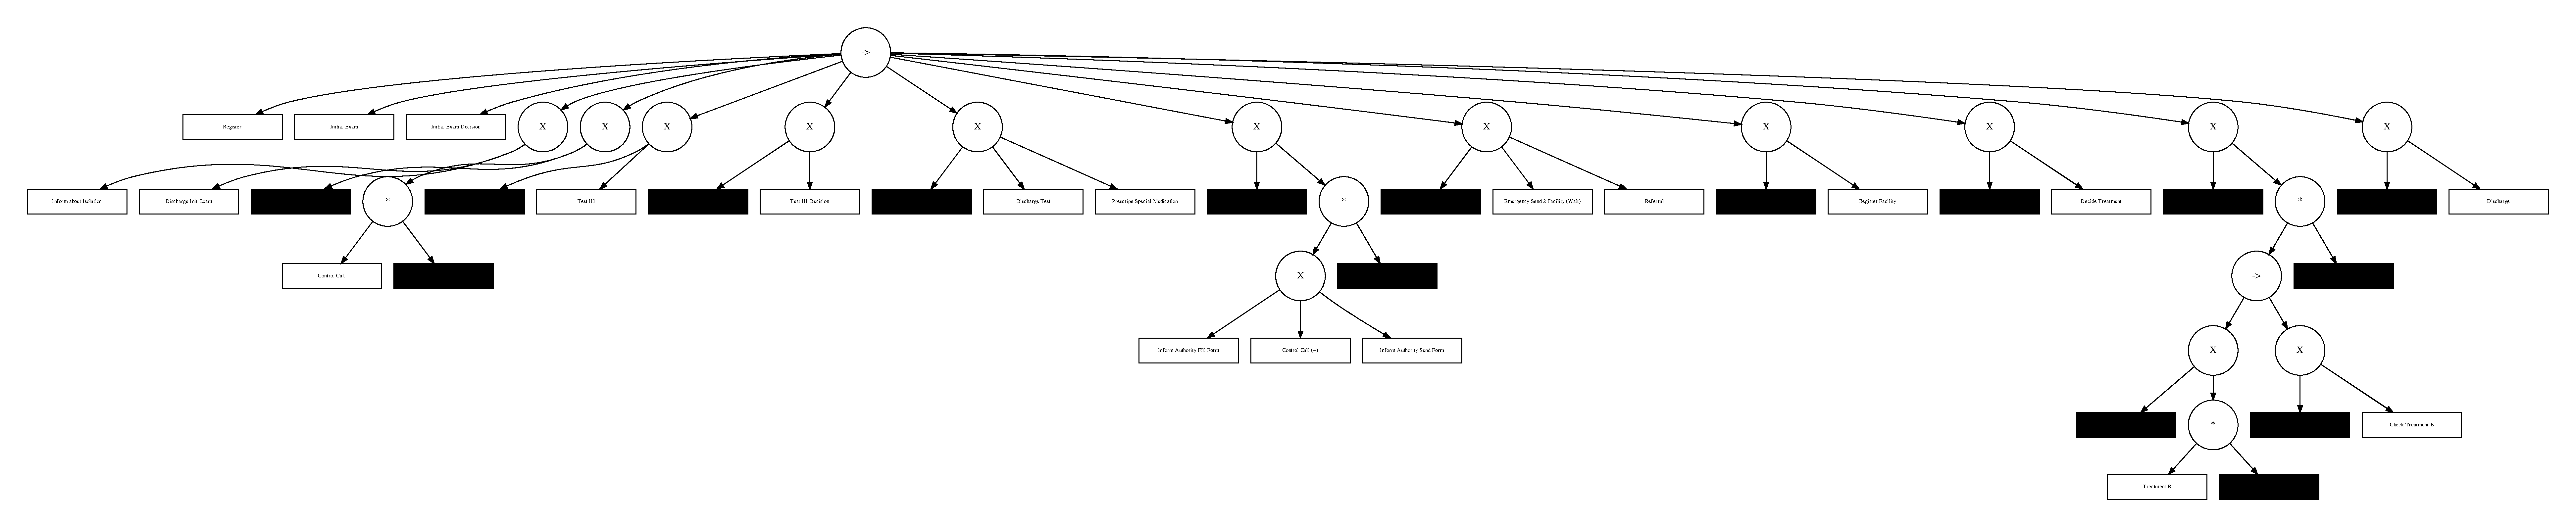
\includegraphics[width=\textwidth]{figures/q1_d_tree_silent_A.pdf}
        \caption{Process Tree}
        \label{fig:figures-q1_d_tree_silent_A-pdf}
    \end{subfigure}
    \hfill
    \caption{Model resulting after the filtering of just the activities related to the A treatments}
    \label{fig:dfg-pt-silent-A}
\end{figure}

The fine tuning of the threshold resulted in the model that can be seen in Figure \ref{fig:noise-threshold-tuning-model}. This approach resulted in a model that represents more behaviors of the event log. The major outcome in the model would be the exclusive choice operator after the \emph{Decide Treatment} activity that distinguished between the treatments.

\begin{figure}[h]
    \centering
    \begin{subfigure}[b]{0.2\textwidth}
        \centering
	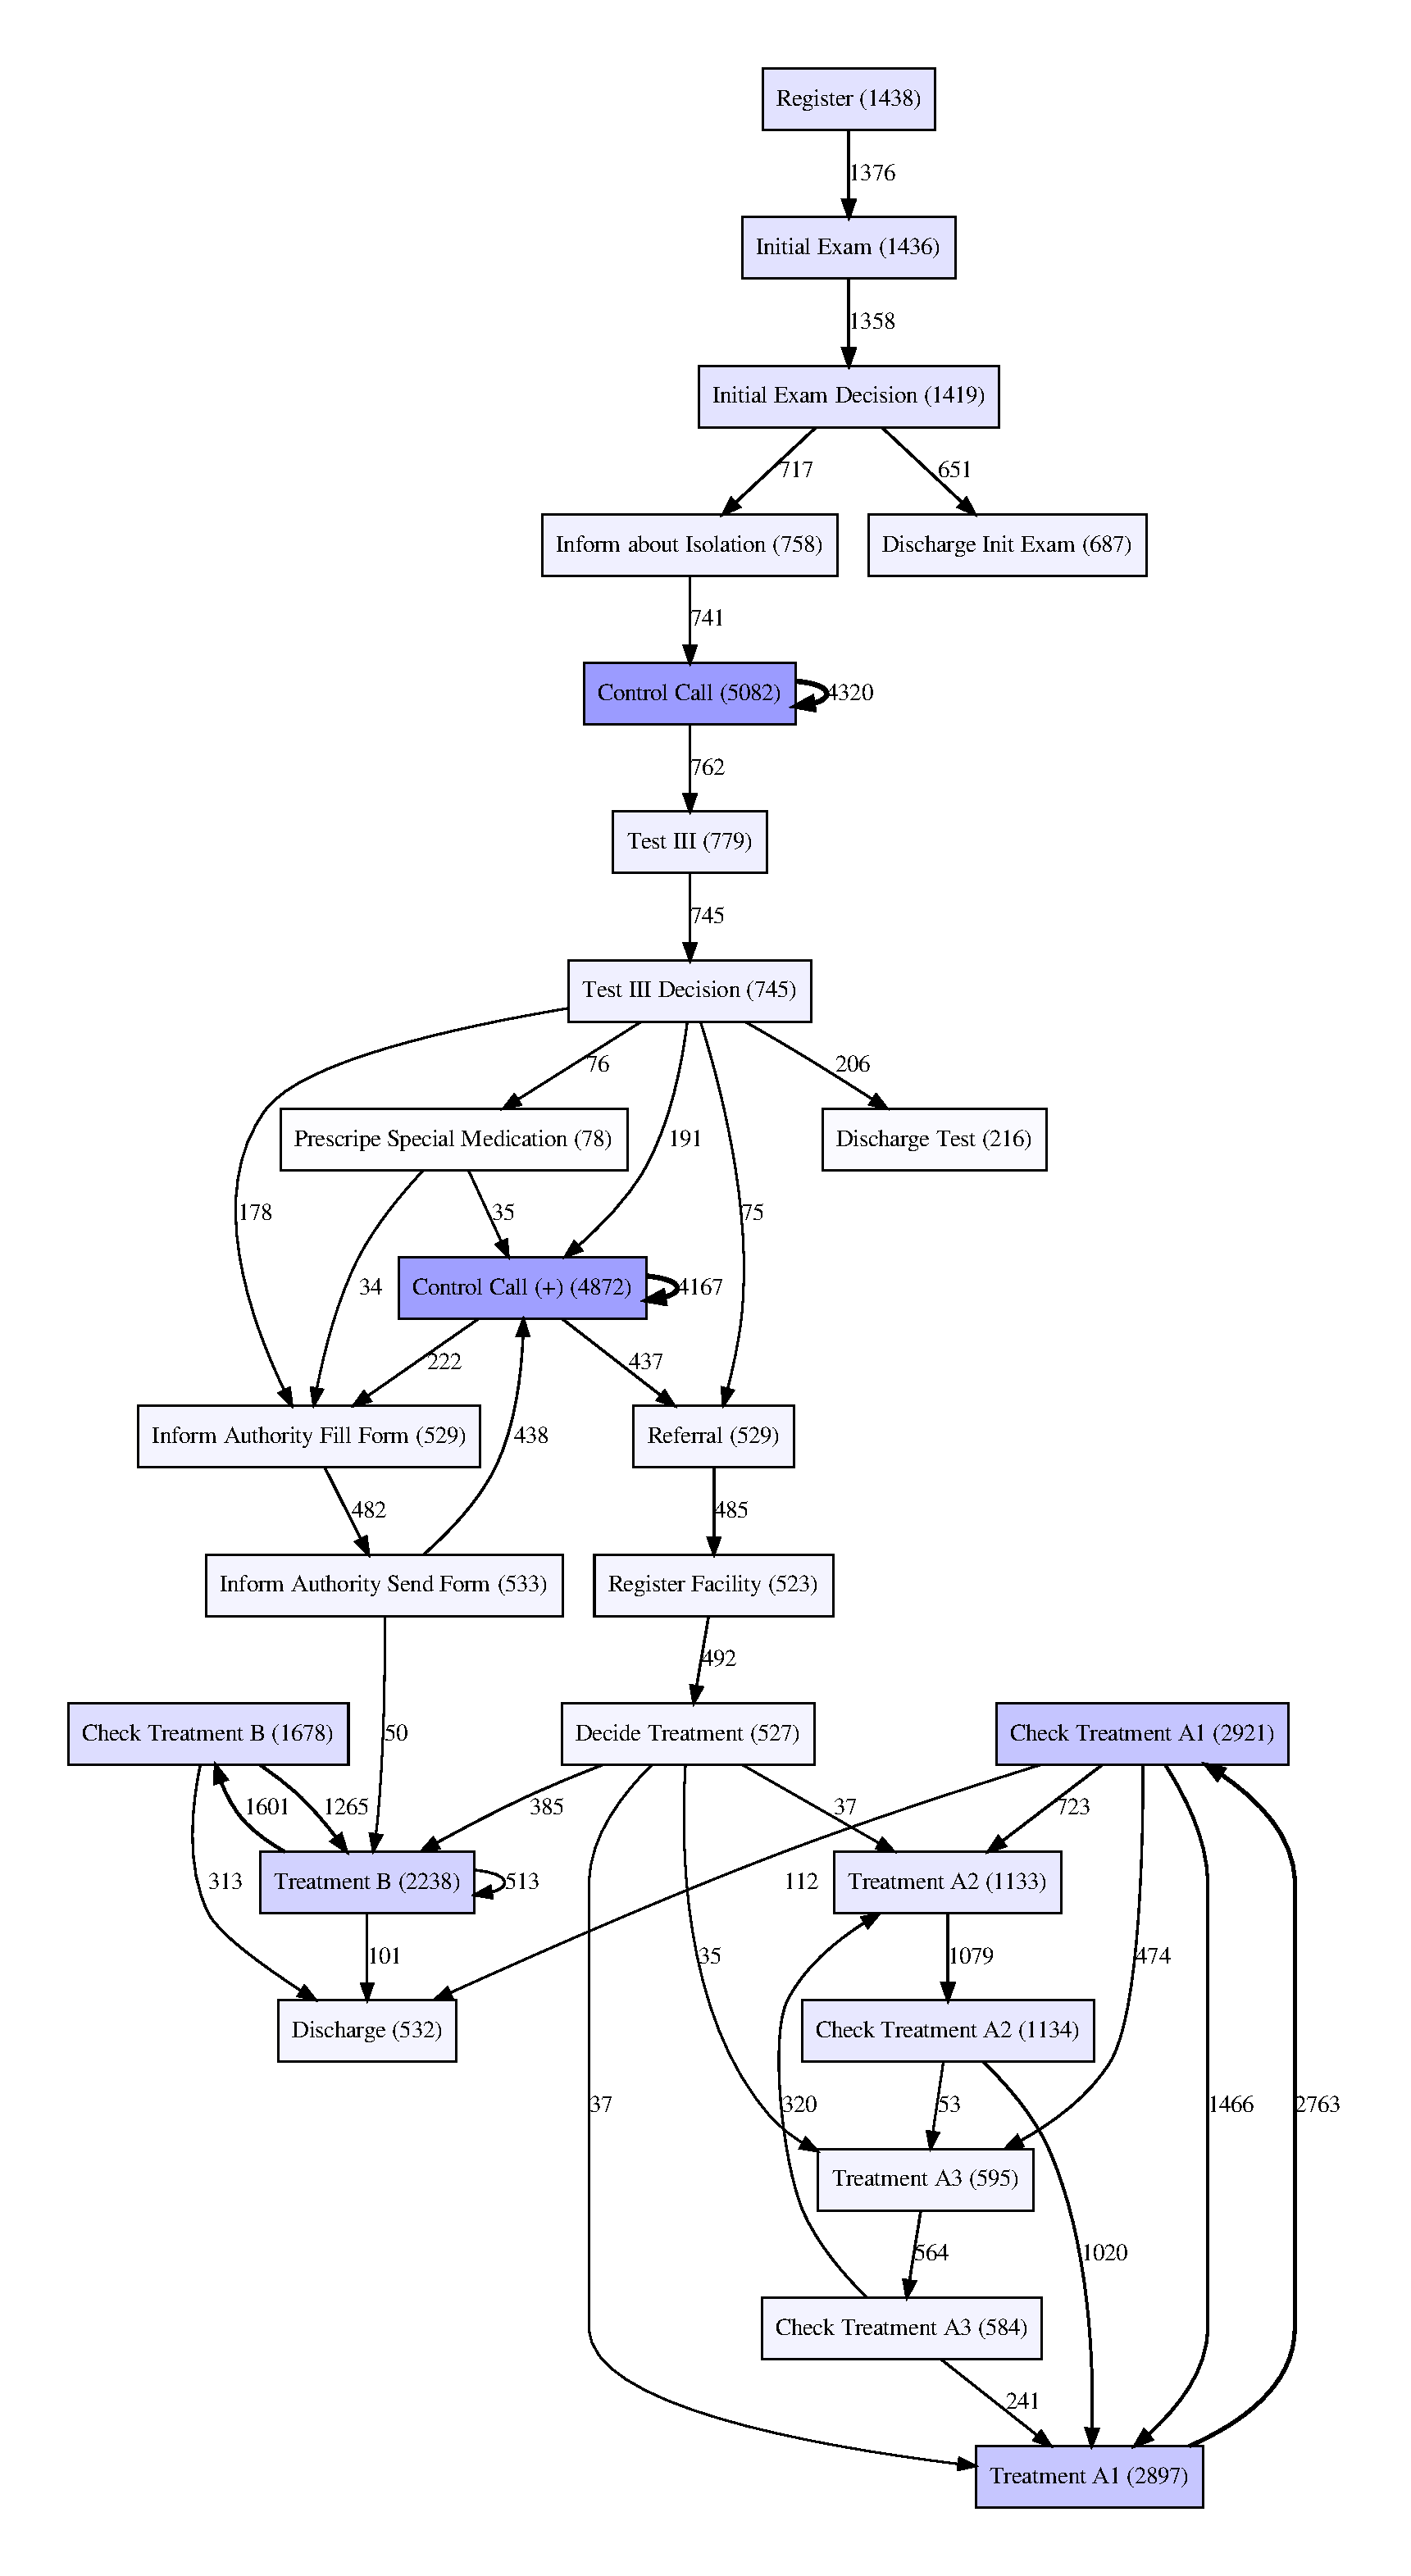
\includegraphics[width=\textwidth]{figures/q1_d_dfg_noise_threshold_tuning.pdf}
        \caption{DFG}
        \label{fig:figures-q1_d_dfg_noise_threshold_tuning-pdf}
    \end{subfigure}
    \hfill
    \begin{subfigure}[b]{0.7\textwidth}
        \centering
	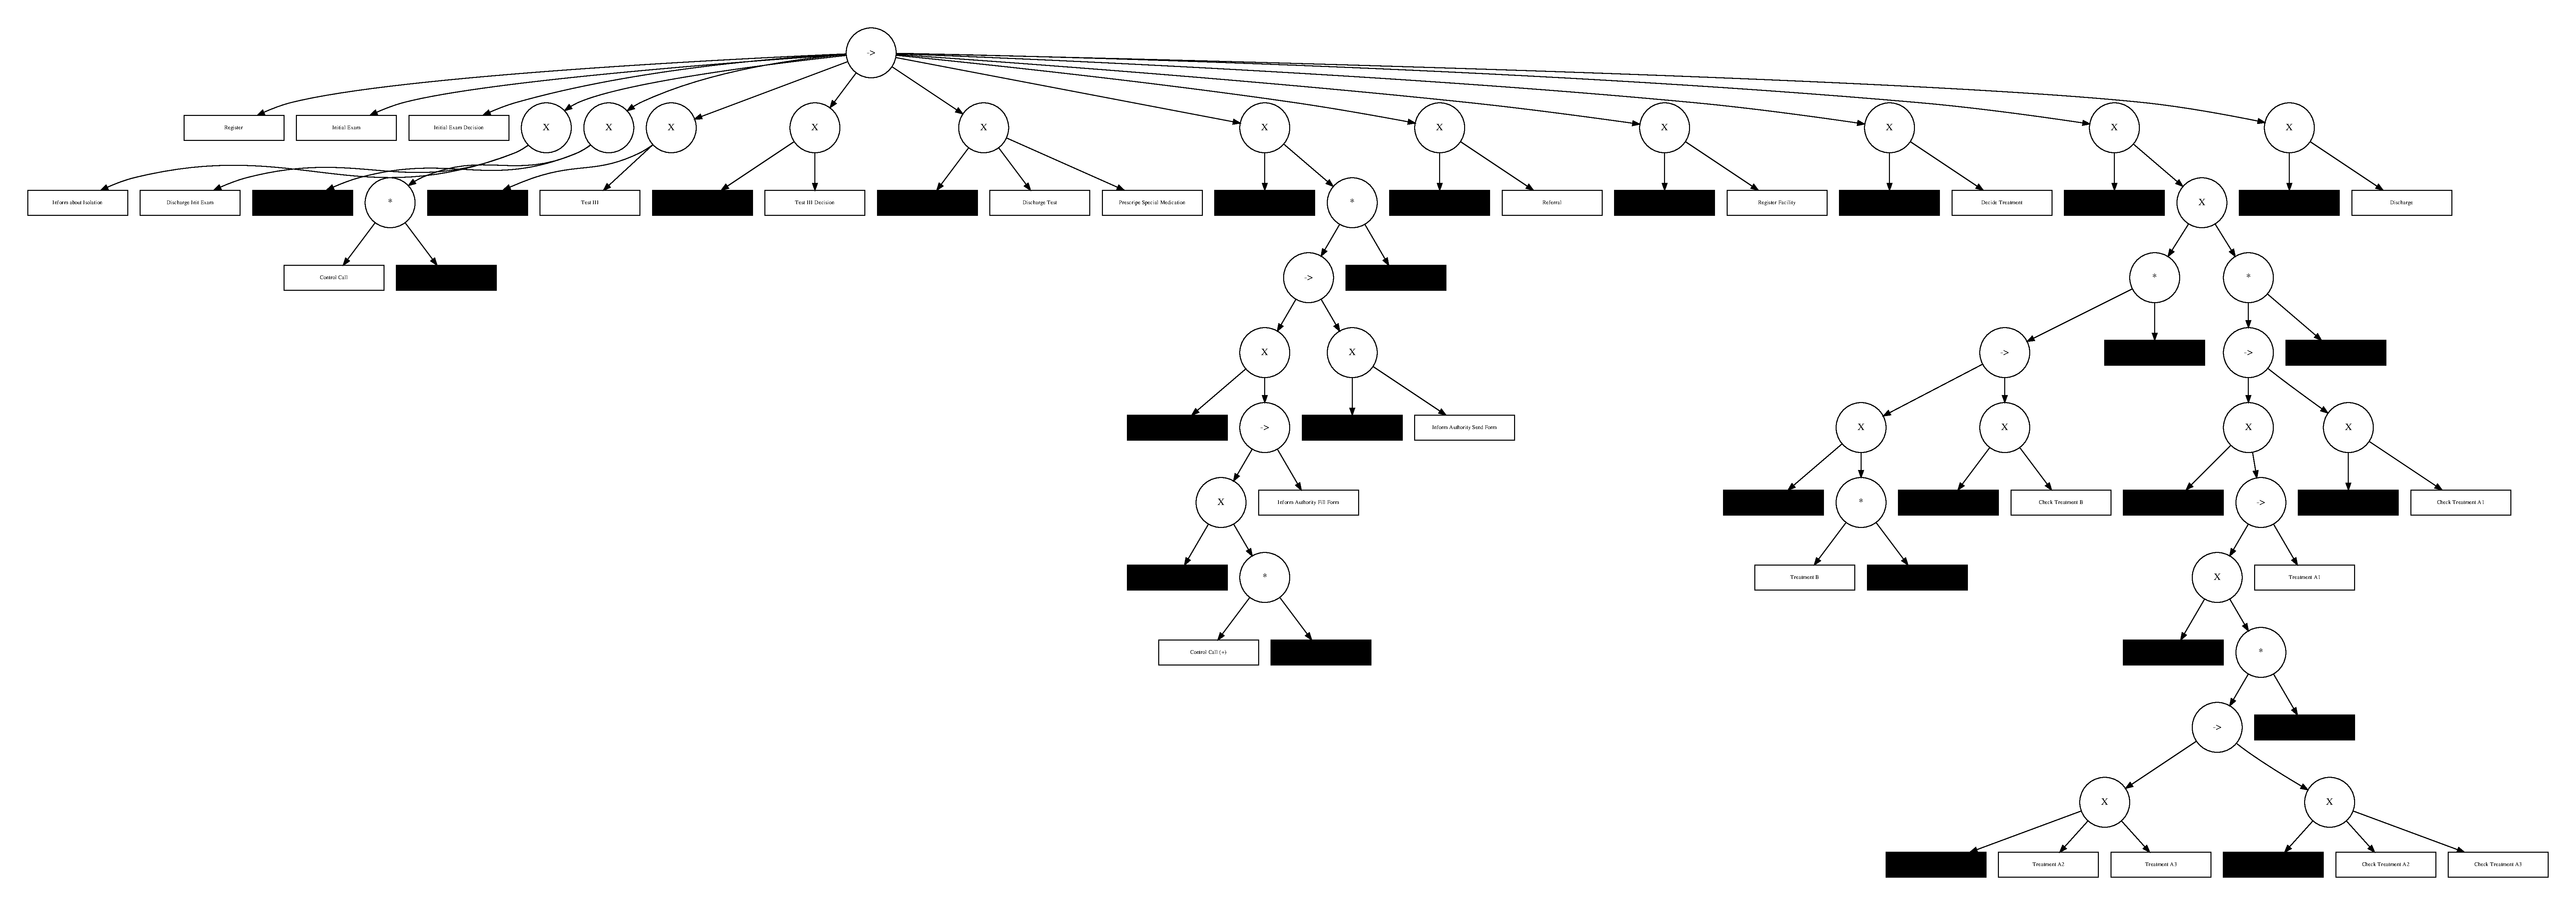
\includegraphics[width=\textwidth]{figures/q1_d_noise_threshold_tuning.pdf}
        \caption{Process Tree}
        \label{fig:q1_d_noise_threshold_tuninig-pdf}
    \end{subfigure}
    \hfill
    \caption{Model resulting from the tuning of the noise threshold}
    \label{fig:noise-threshold-tuning-model}
\end{figure}

\paragraph{e)} 

Analysing the traces in which this activity occur we reinforce what was noted above and estimate that the special medication is prescribe only to patients that go through the A treatments, therefore reasoning its total absence from the model where these traces were filtered out. To try and understand this better, we modeled only these traces that were left out from the aforementioned model. The result can be seen in Figure \ref{fig:special-medication-model}. Besides what was already discussed, one can say that the previous models failed to capture the non-local influence of this activity, which is expected for the Inductive Mining algorithm.

\begin{figure}[h]
    \centering
    \begin{subfigure}[b]{0.2\textwidth}
        \centering
	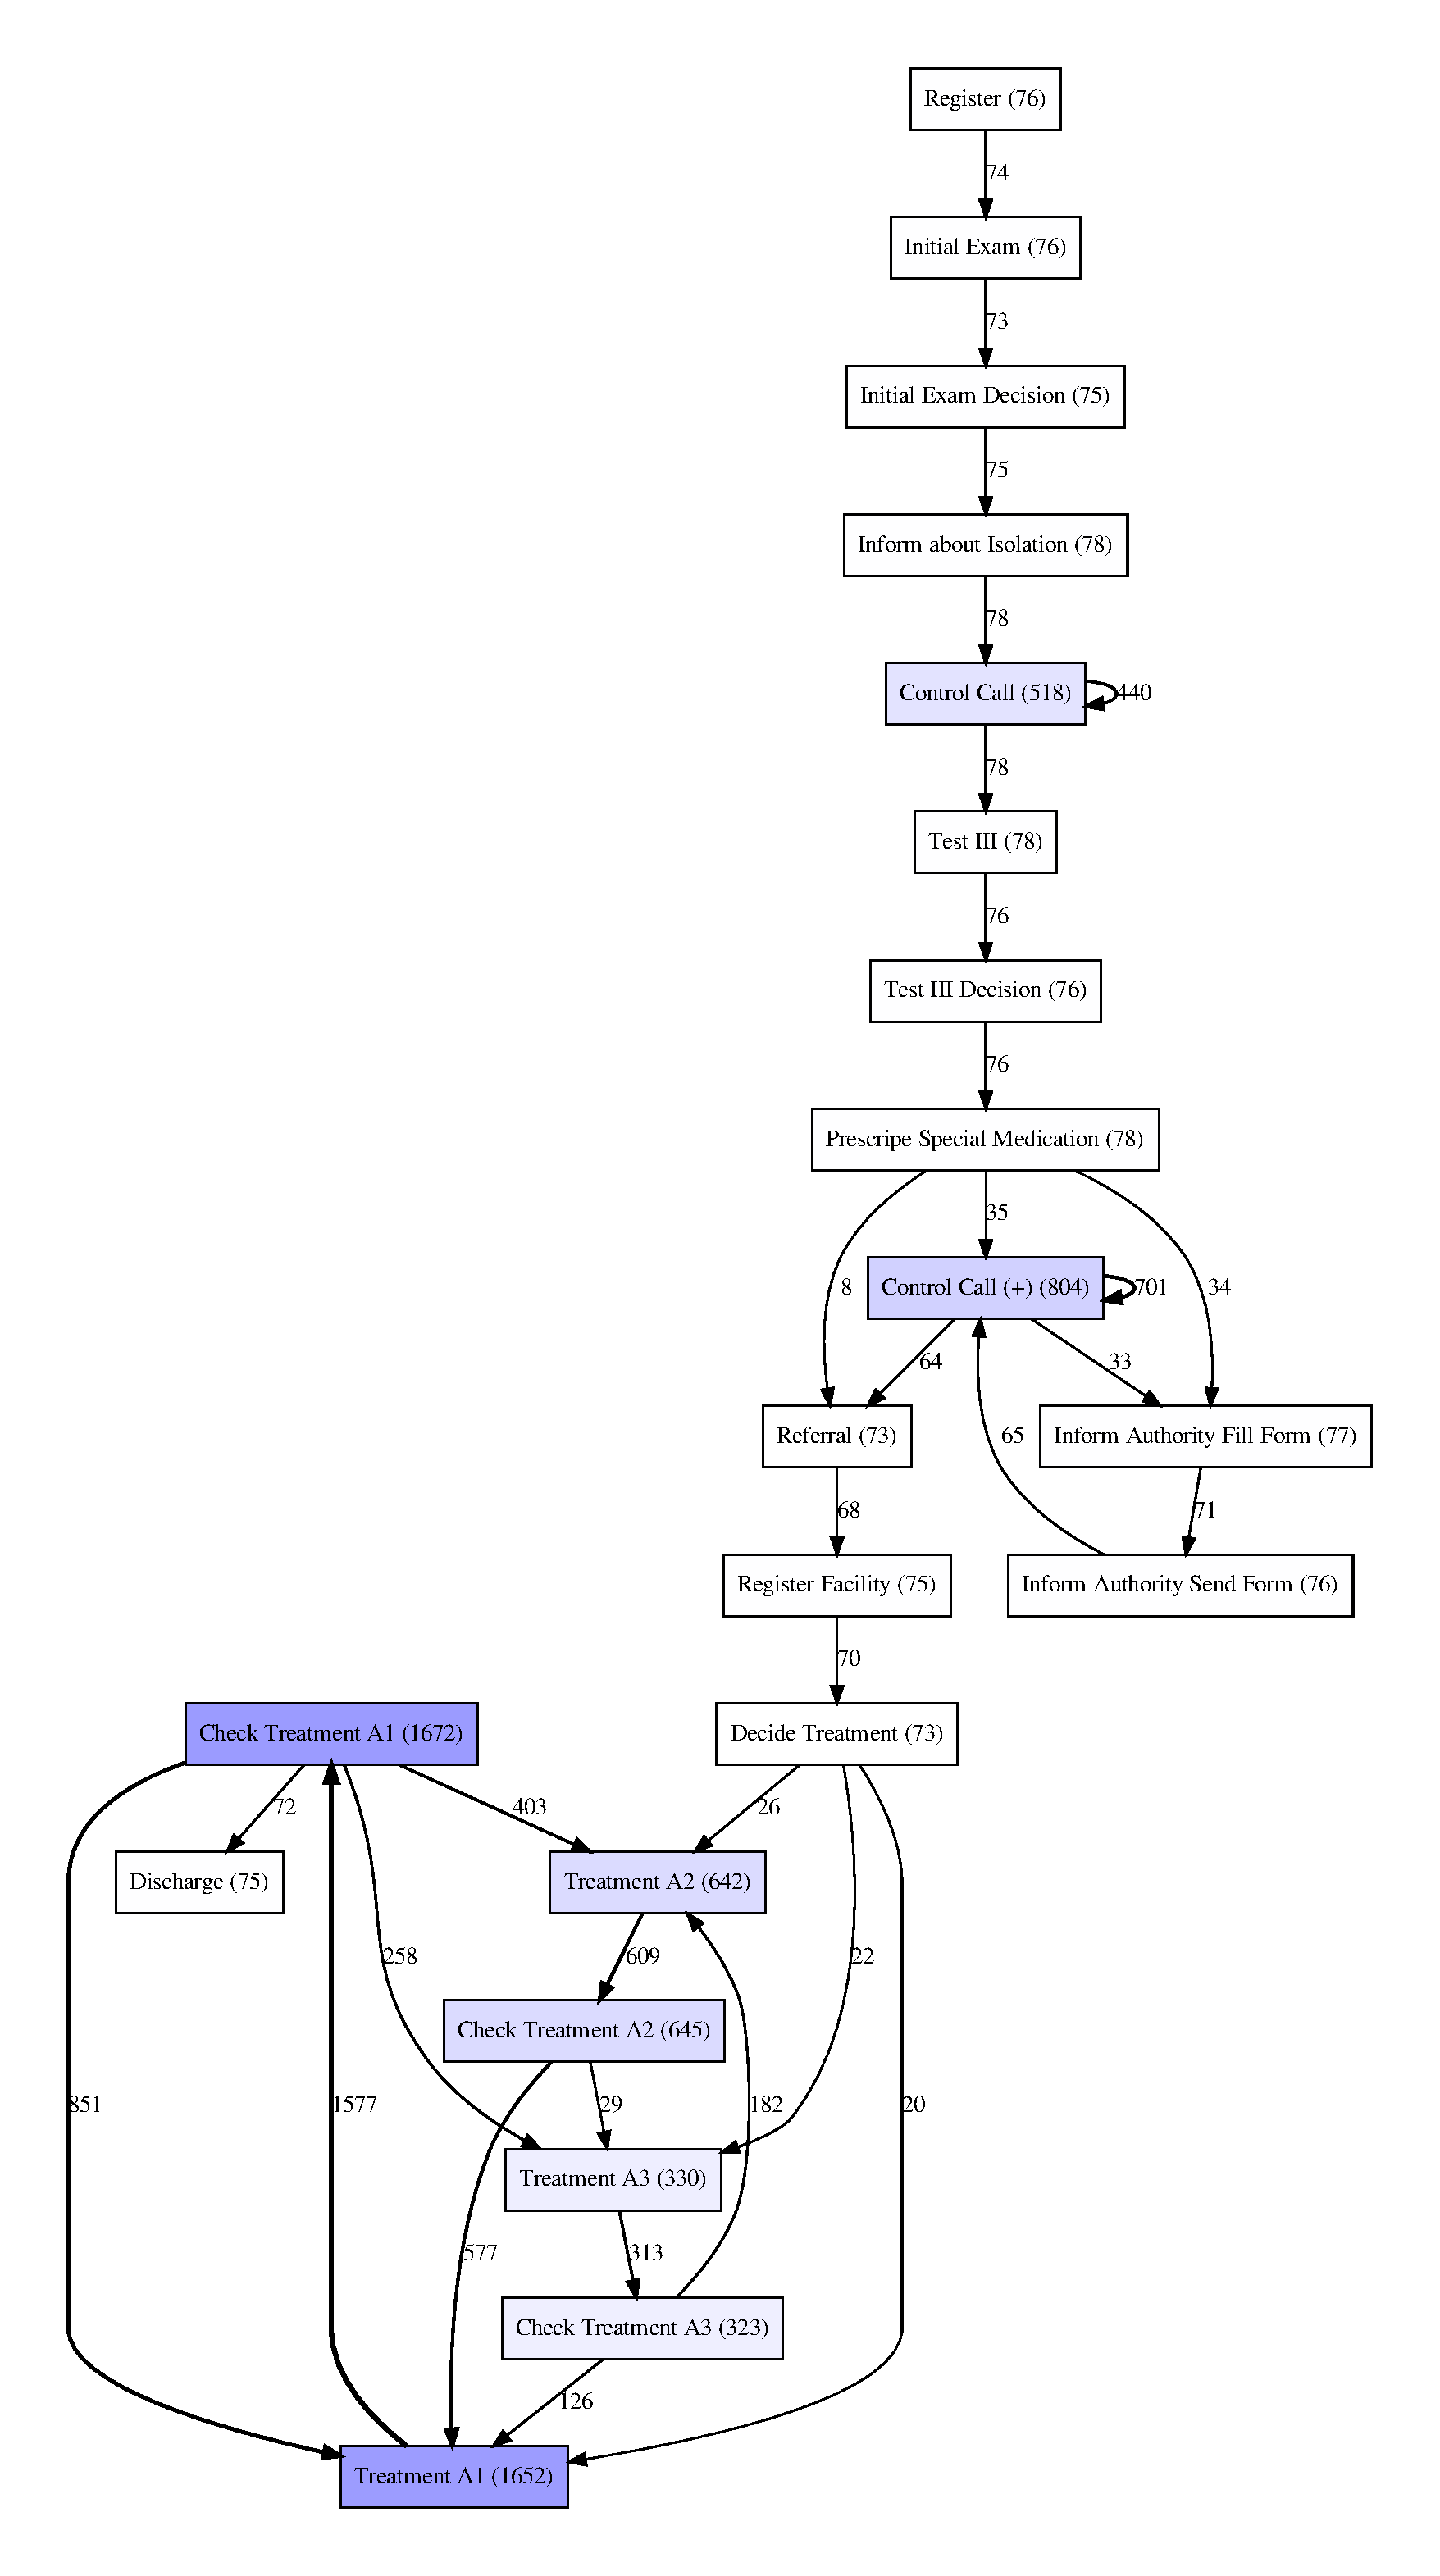
\includegraphics[width=\textwidth]{figures/q1_e_special.pdf}
        \caption{DFG}
        \label{fig:figures-q1_e_special-pdf}
    \end{subfigure}
    \hfill
    \begin{subfigure}[b]{0.7\textwidth}
        \centering
	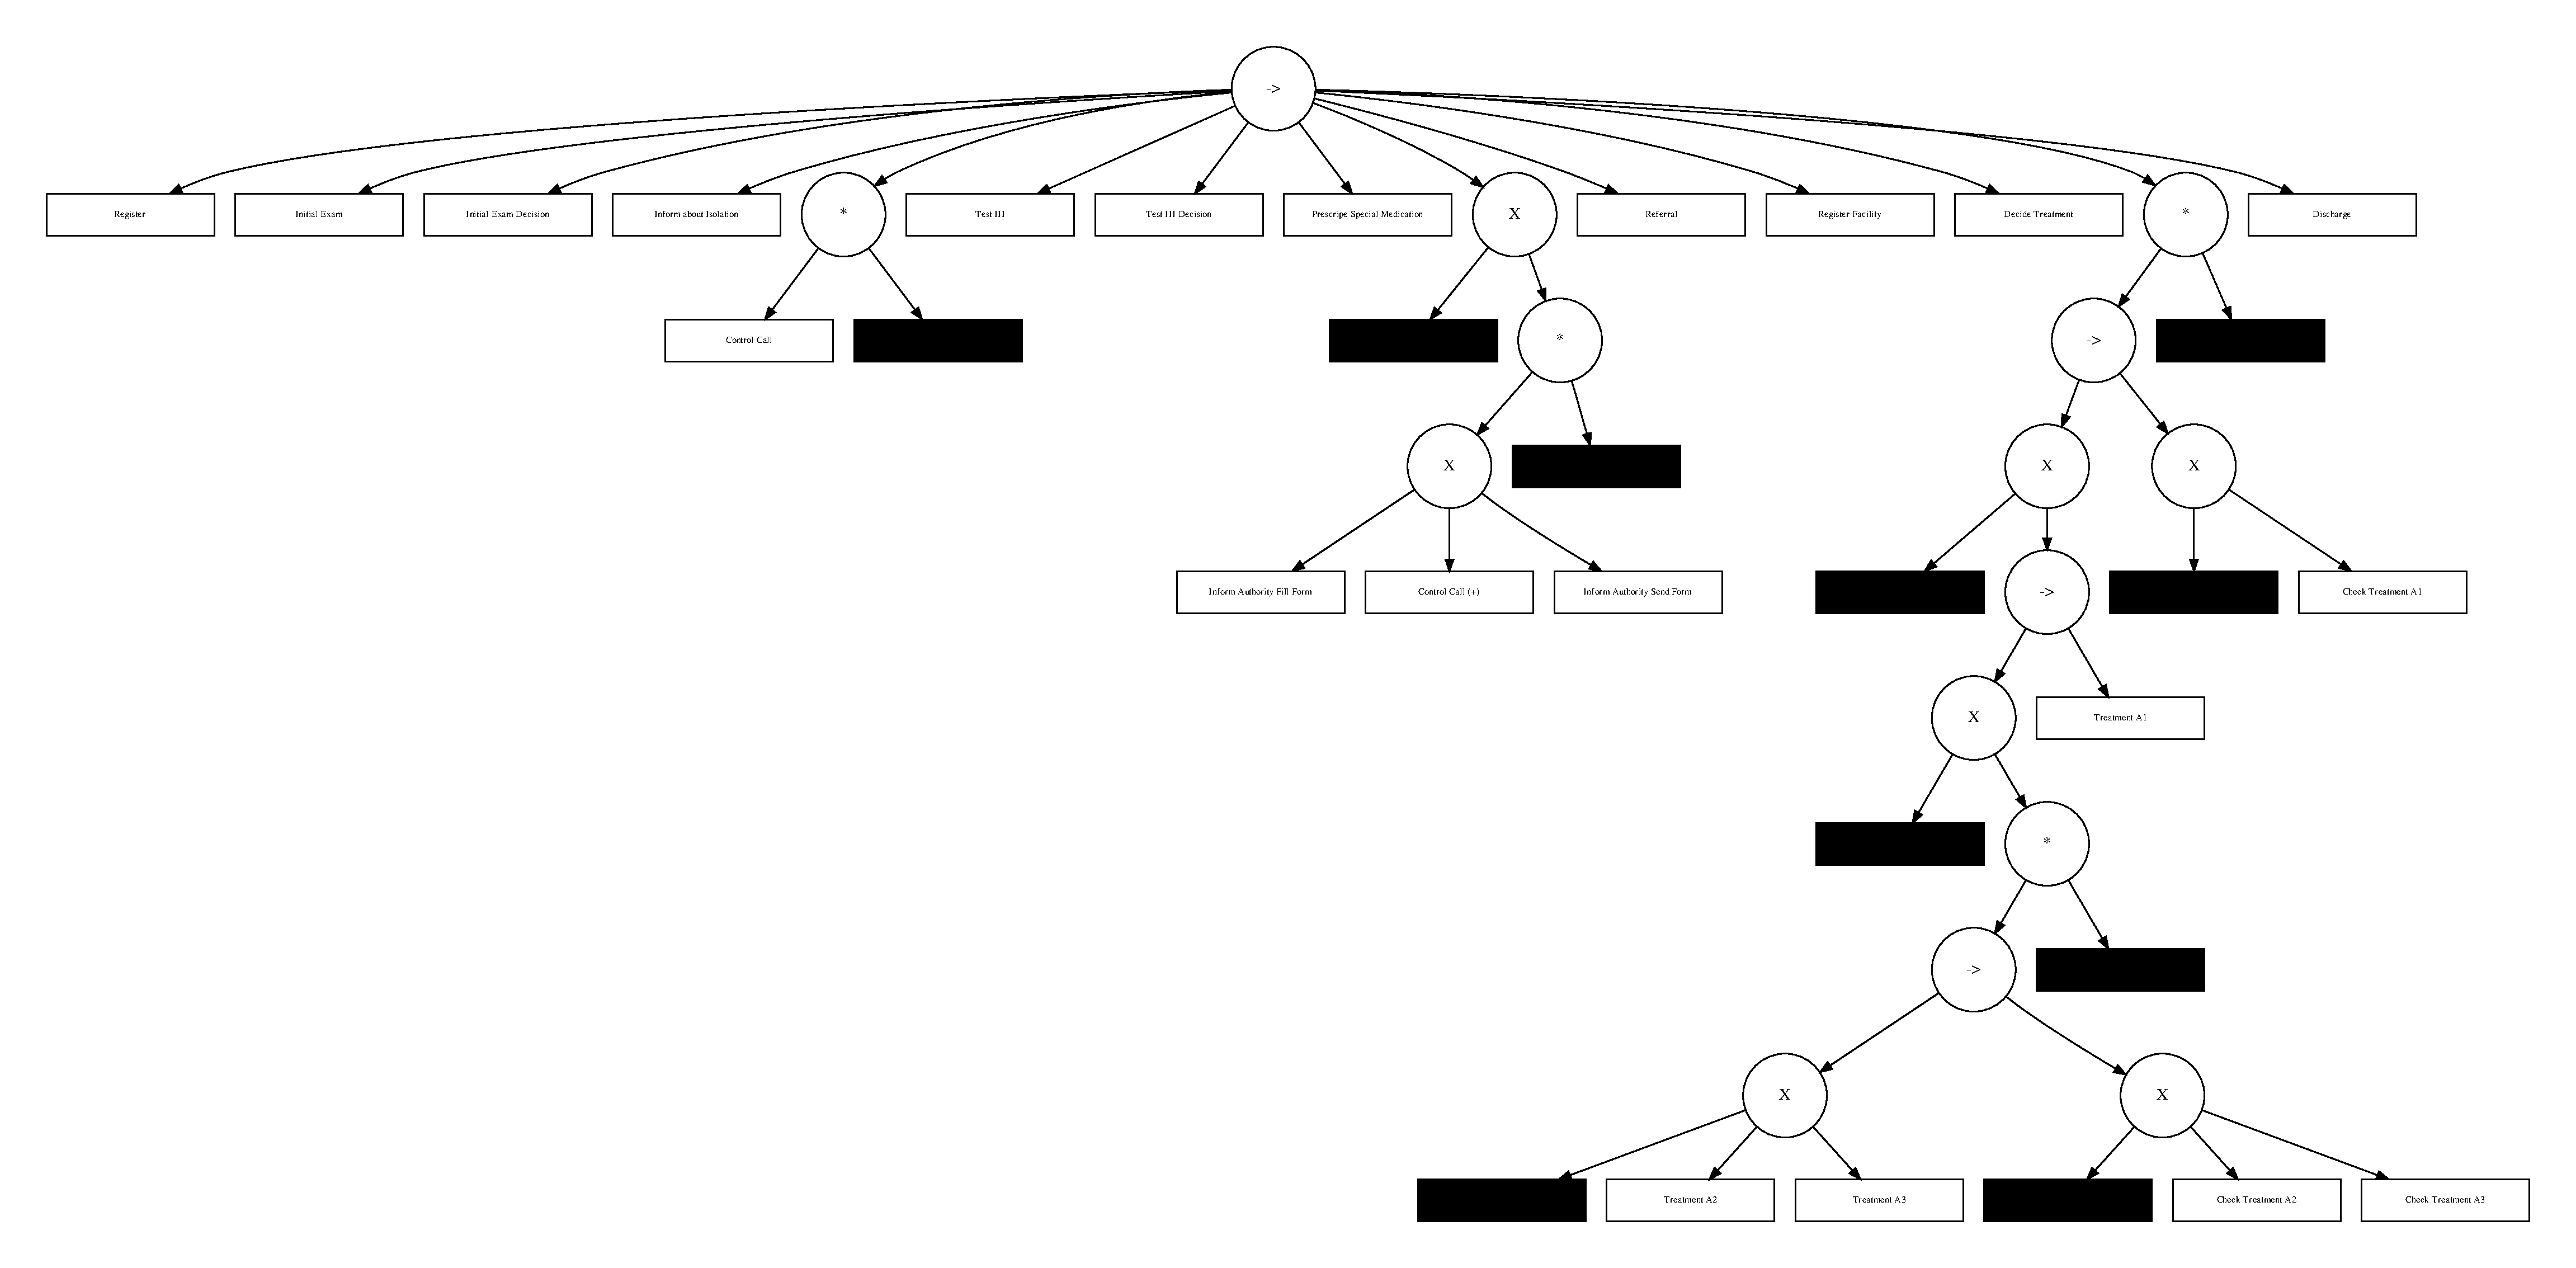
\includegraphics[width=\textwidth]{figures/q1_e_tree_special.pdf}
        \caption{Process Tree}
        \label{fig:q1_e_tree_special-pdf}
    \end{subfigure}
    \hfill
    \caption{Model resulting from event log containing only the traces in which the \emph{Prescripe Special Medication} was present}
    \label{fig:special-medication-model}
\end{figure}

\paragraph{f)} 

The Alpha Miner and the Heuristics Miner algorithms were applied to the event log. The resulting model from the AM can be seen in Figure \ref{fig:figures-q1_f_alpha_miner-pdf}. We can see that the resulting Petri Net fails to model most of the behaviors of the process, having several loose transitions and even failing to be an workflow net.

\begin{figure}[h]
    \centering
    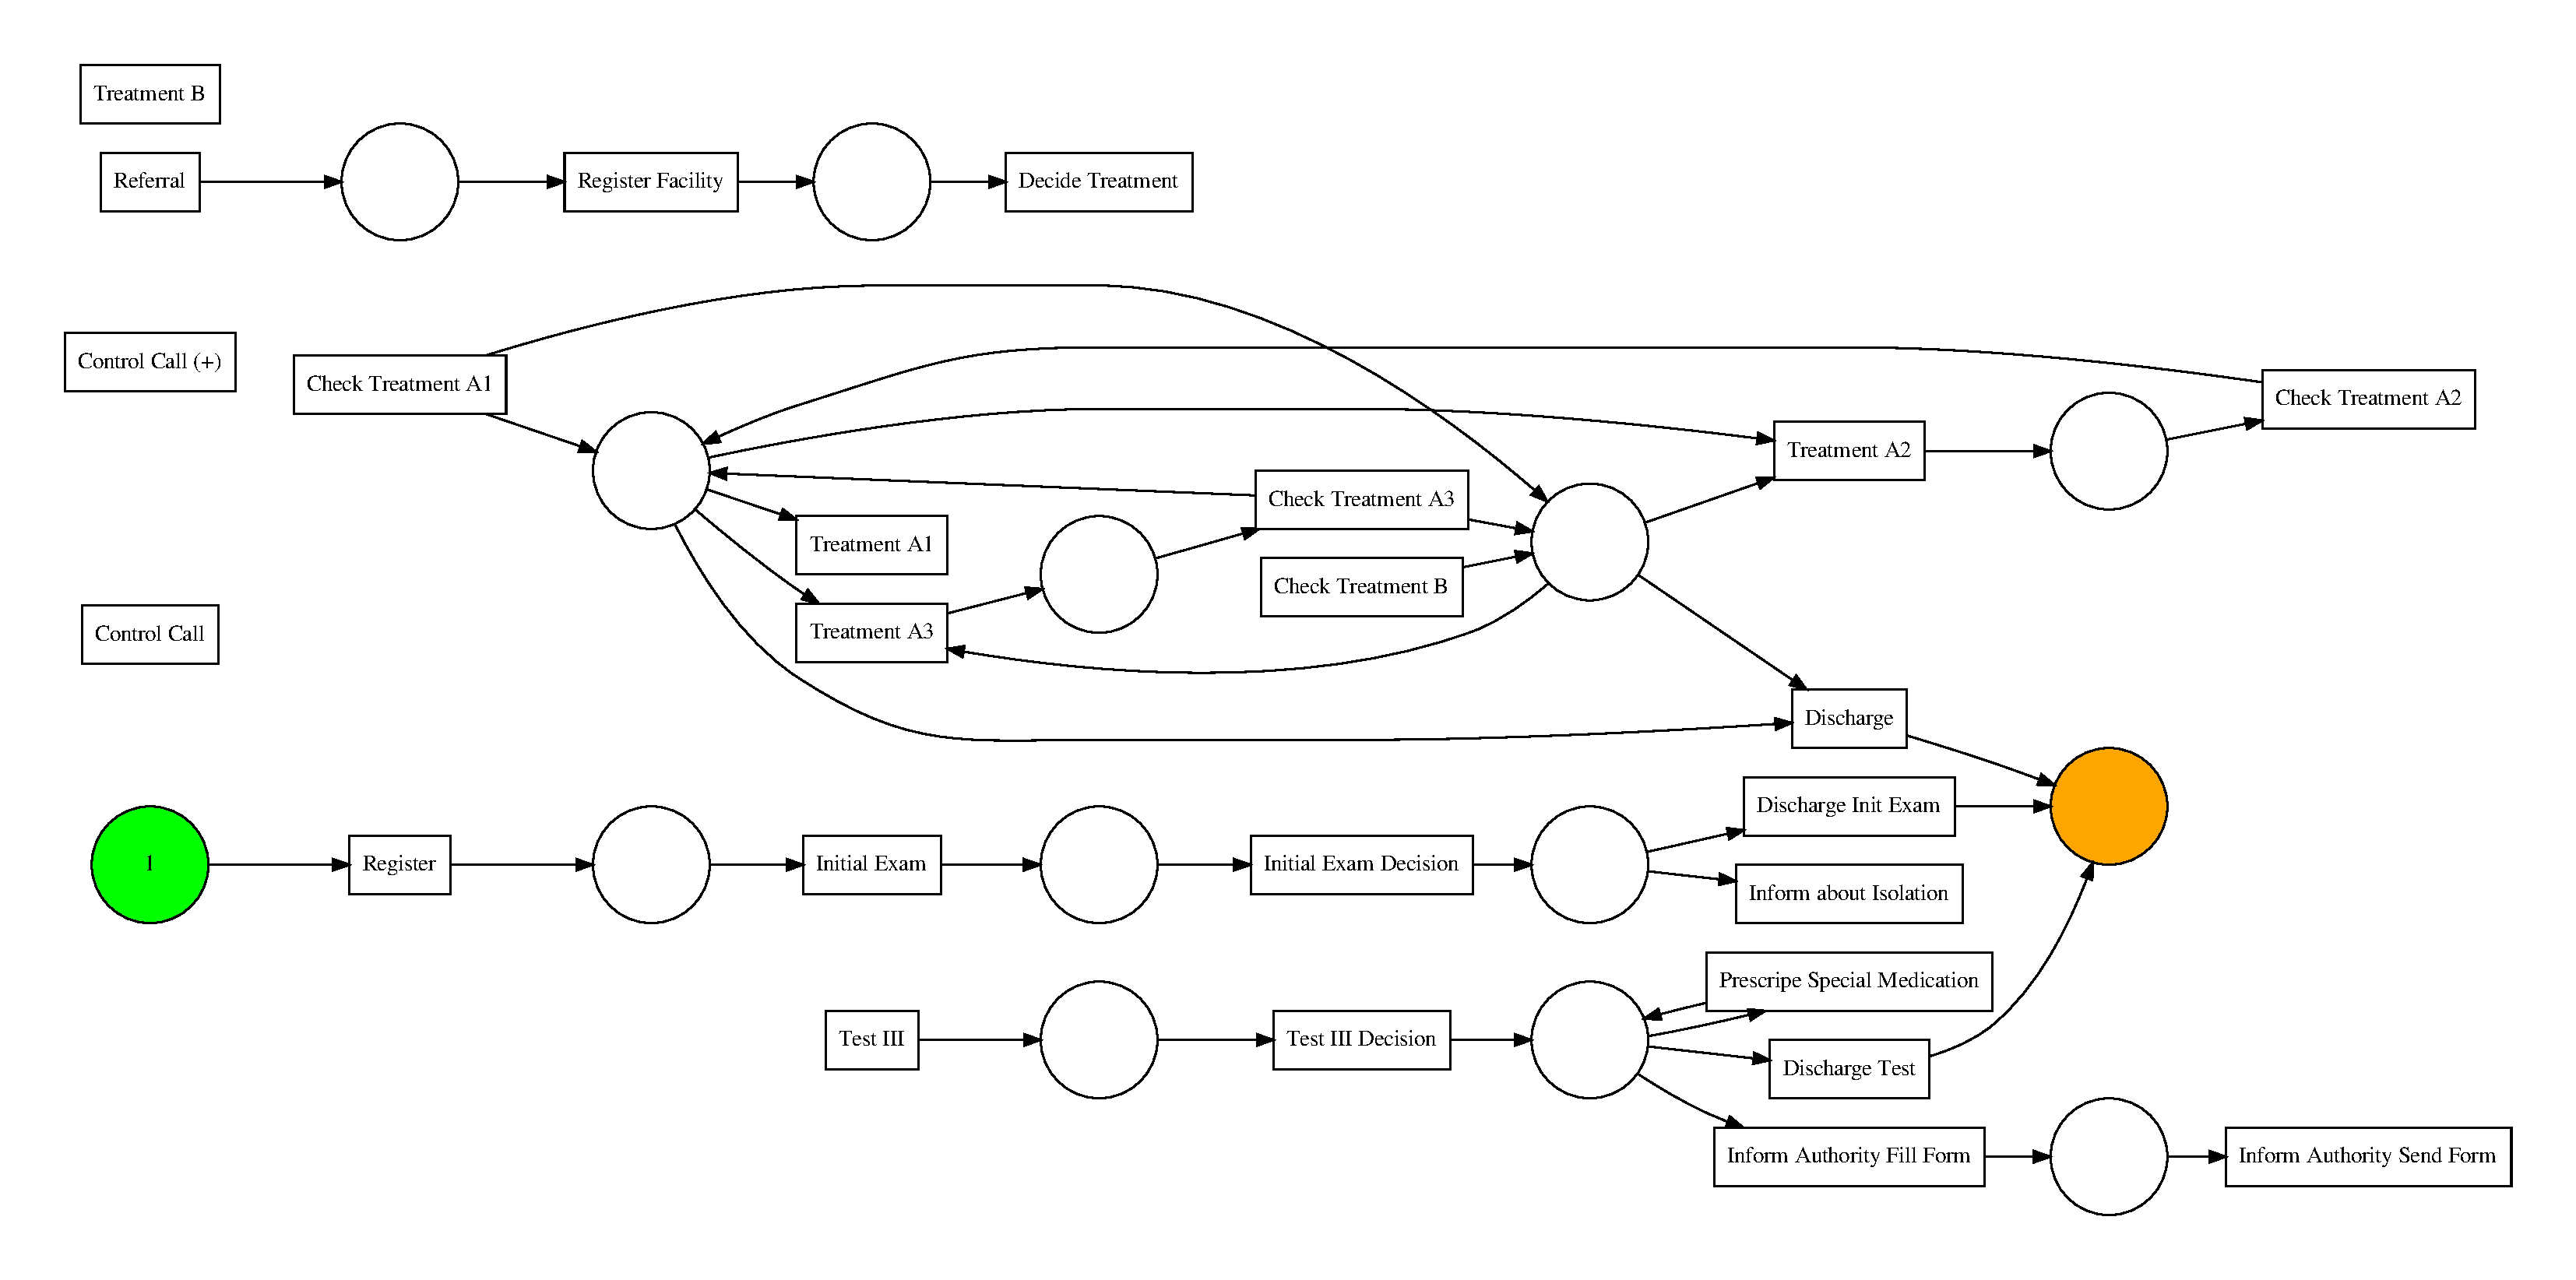
\includegraphics[width=\textwidth]{figures/q1_f_alpha_miner.pdf}
    \caption{Petri Net resulting from the Alpha Miner application to the event log}
    \label{fig:figures-q1_f_alpha_miner-pdf}
\end{figure}

The results of the HM application can be seen in Figure \ref{fig:figures-q1_f_heuristics_miner-pdf}. It presents a satisfactory modeling of the initial activities and even some of the more complex behaviors as the first \emph{Control Call} and the split after the test. But it also fails to model the non-local influence of the \emph{Prescripe Special Medication} activity and the relation between the treatment activities. We also notice that the model is not sound, allowing for the overflow of tokens in some places through silent transitions. Perhaps the biggest problem of this model is related to the activities related to the treatment, where it fails to model the behavior almost completely.

\begin{figure}[h]
    \centering
    
\includegraphics[width=\textwidth]{figures/q1_f_heuristics_miner.pdf}
    \caption{Petri Net resulting from the Heuristics Miner application to the event log}
    \label{fig:figures-q1_f_heuristics_miner-pdf}
\end{figure}

For these, we can conclude that the Inductive Miner presented the best model out of the 3 algorithms tried.

\section{Q2. Social Network Analysis}
\textlangle Optional: Introduction \textrangle
\paragraph{a)} 

A handover-of-work network connects two resources when an activity performed by one resource directly follows the activity performed by another resource. The more frequent this relationship is in the log, the higher is the weight of an edge. In the Figure \ref{fig:figures-q2_handover-png} below the handover-of-work network that was discovered from the given log can be seen.

\begin{figure}[h]
    \centering
    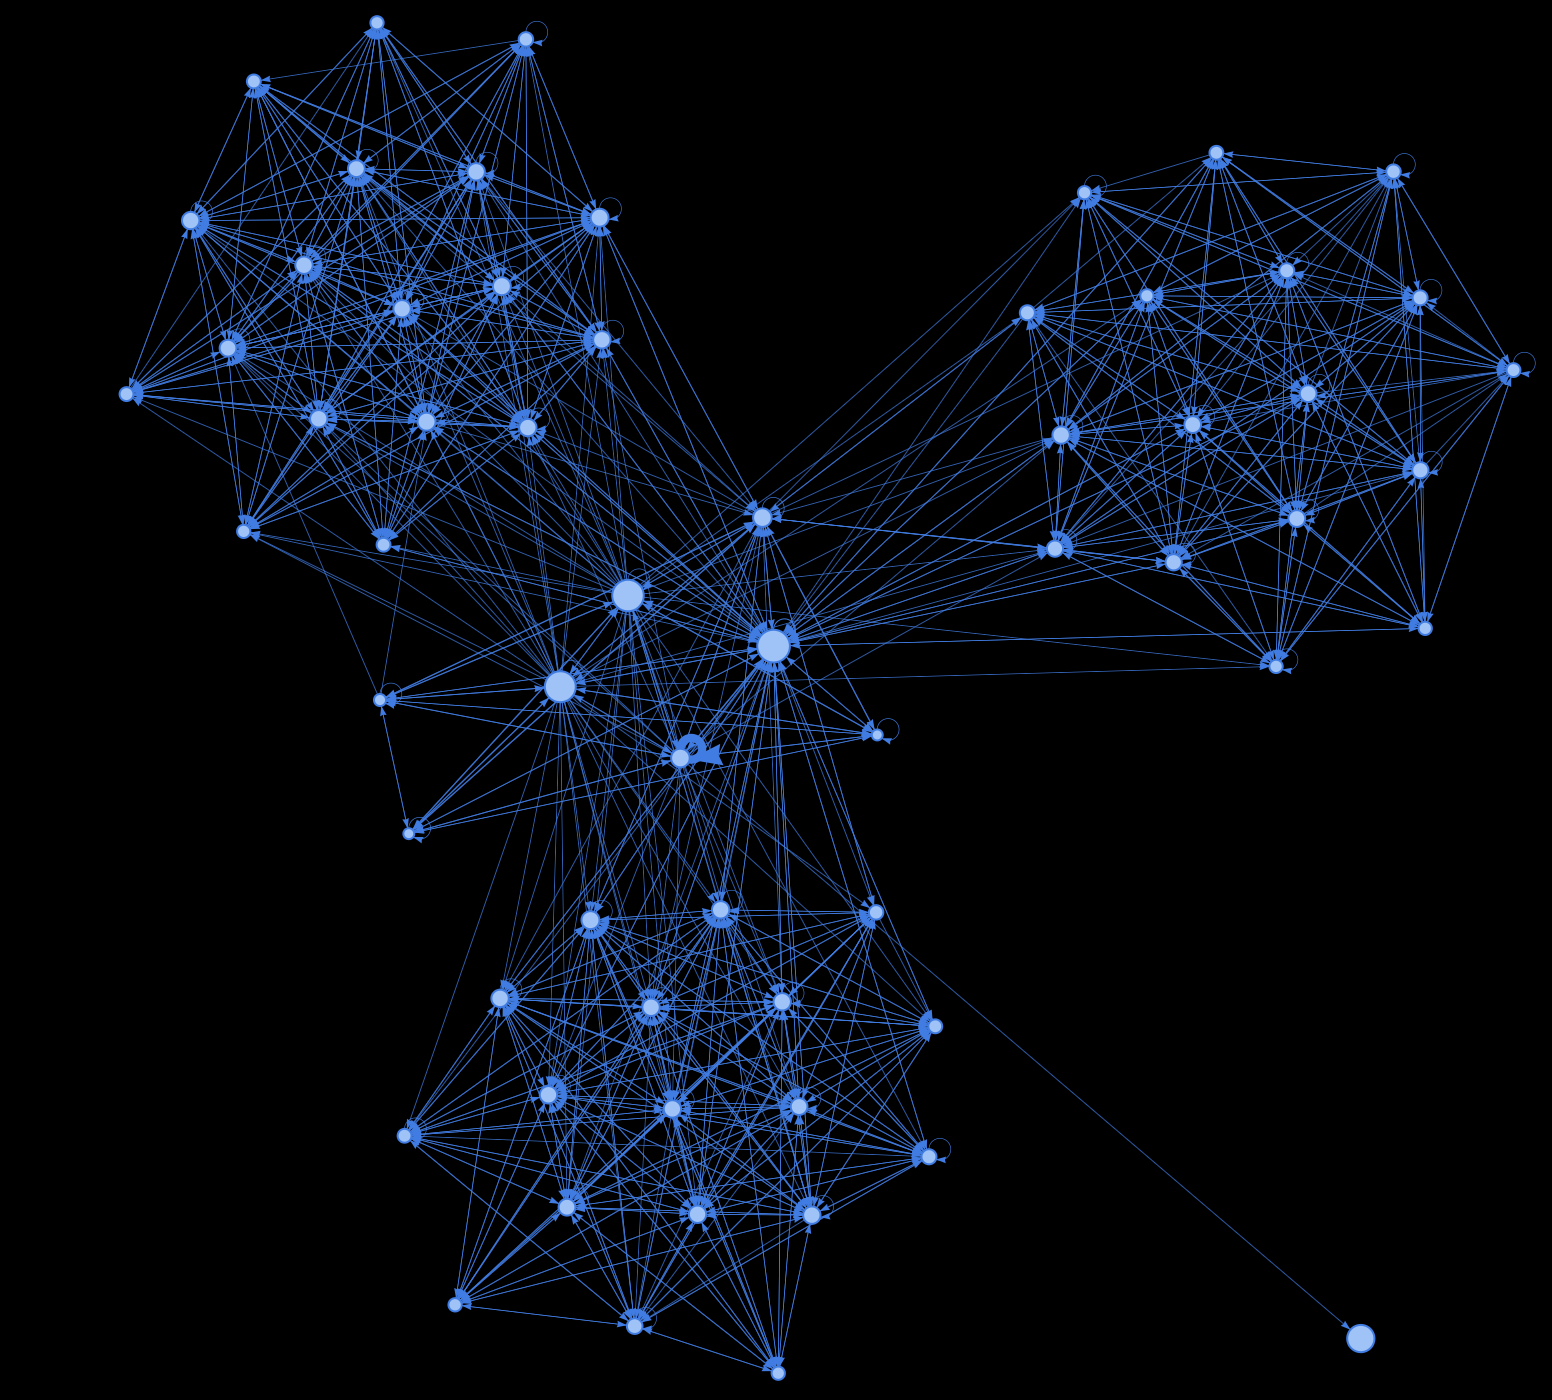
\includegraphics[width=0.6\textwidth]{figures/q2_handover.png}
    \caption{Handover-of-work network discovered through PM4Py}
    \label{fig:figures-q2_handover-png}
\end{figure}

We see that the network consists of four strongly connected main components and a single resource that has only one connection. Further we see that the resources in each of the strongly connected components all have a common first letter. The outer three components contain resources with first letters B, C and D. The inner component consists of resources with the first letter A. Throughout the rest of this report these components will be referred to by these letters. The nodes in the three outer components are connected only to themselves and the inner A component, but not to the other outer components. Most of the nodes in the A component have connections to all other components and the nodes in the A component have overall the most connections to other nodes. There is a single resource that does not belong to any of the components and has only one incoming edge.

From an organizational perspective the observed network might be explained in the following way: The outer components B, C, D all represent certain distinct departments. All of the resources in such a department do similar work and its members are working together on a certain part of the process. The central A component, however, consists of resources that are delegating and inspecting work. They pass process instances from one department to another. Since the singular resource has only incoming edges, it must be concerned with the end of the process. It might be a kind of supervisor role that makes a final assertion of a process before it ends. However this node is not involved in most cases, as its connection is rather weak.

\paragraph{b)} 

A subcontracting social network visualizes what resources are involved in the work of another resource.

The obtained network that can be seen in Figure \ref{fig:figures-q2_subcontracting-png} has a kind of forest structure. We again see distinct connected components that show the same A, B, C, D division as in the handover-of-work network discussed above. There is one component for each of these, except for the A component, which now consists of two not connected components. As a common structure we can observe a kind of star pattern for many nodes, meaning that one resource is involved in the work of many other resources. We can see that one of the A components has a very strong relation between two of the resources.

\begin{figure}[h]
    \centering
    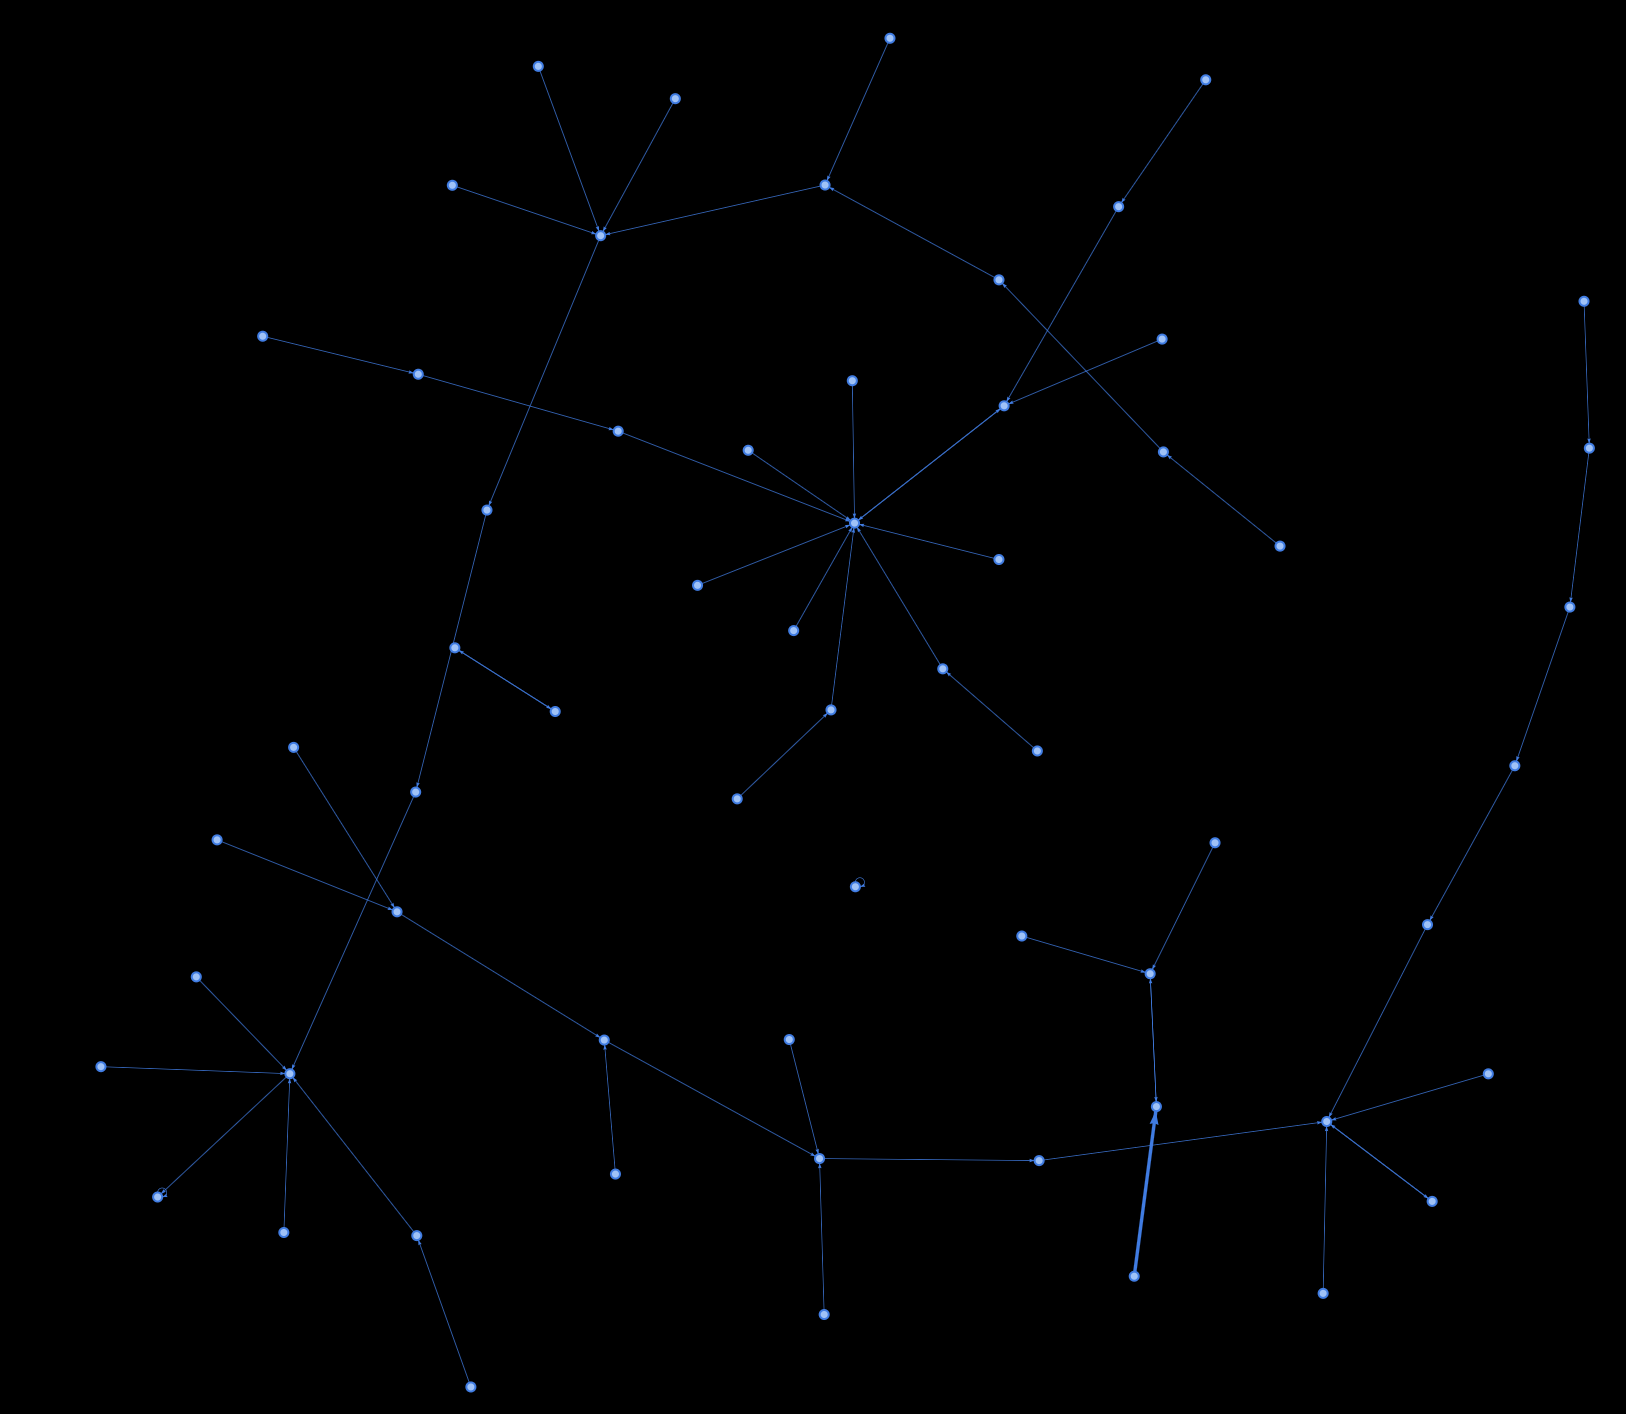
\includegraphics[width=0.6\textwidth]{figures/q2_subcontracting.png}
    \caption{Subcontracting network discovered through PM4Py}
    \label{fig:figures-q2_subcontracting-png}
\end{figure}

From an organizational perspective we can again see that the work of one department never involves the work of another department. Subcontracting only happens within the A, B, C, and D departments. The star structures suggest that there are supervisor roles, resources that often subcontract work to other resources which do not subcontract any work. The strong connection between the \emph{Alexander} and \emph{Ava} resources suggests that the first is in a leadership position and the second might be a related secretary, as most of the work is subcontracted.

\paragraph{c)} 

A working-together network depicts which resources are often working together on the same case, so in which fraction of cases they were both involved. The generated network can be seen in Figure \ref{fig:figures-q2_working_together-png}.

\begin{figure}[h]
    \centering
    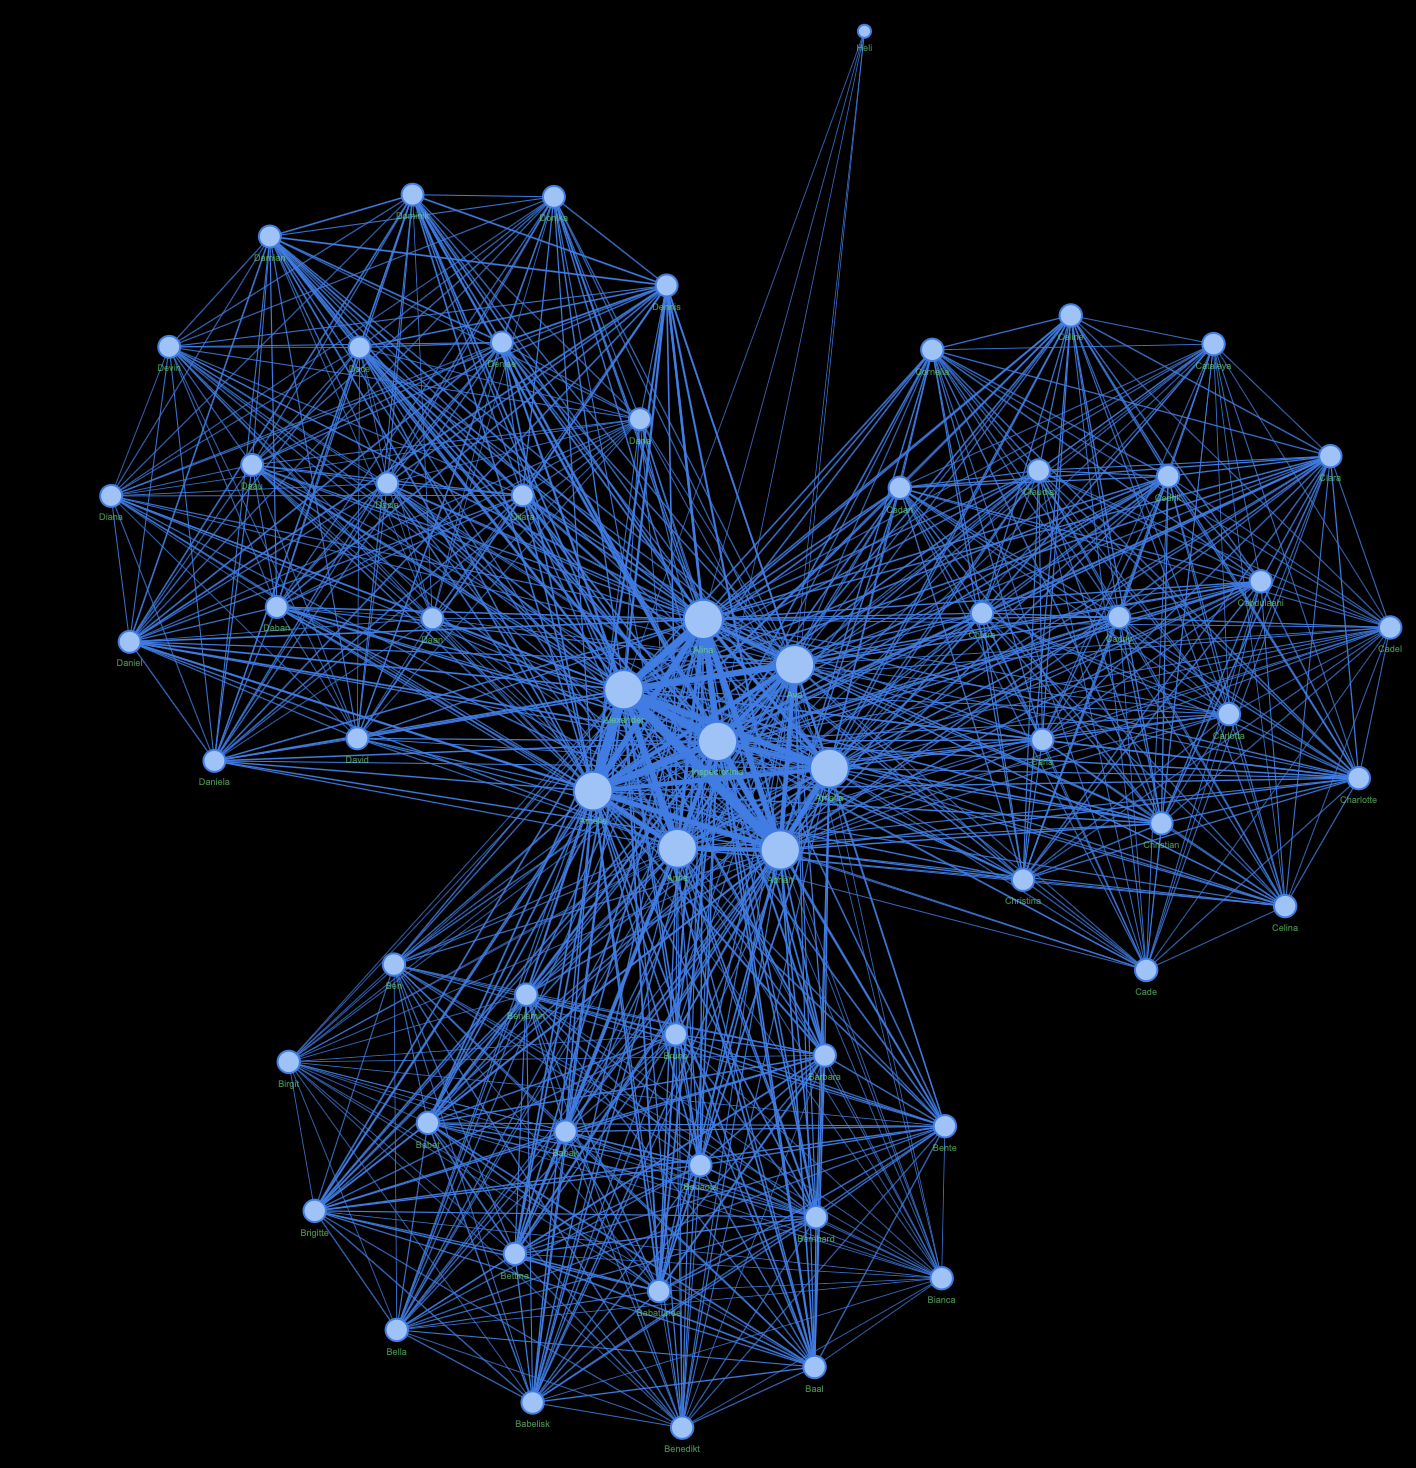
\includegraphics[width=0.6\textwidth]{figures/q2_working_together.png}
    \caption{Working-together network generated through PM4Py}
    \label{fig:figures-q2_working_together-png}
\end{figure}

We see a similar structure as in the handover-of-work network, which is expected from our previous assumptions. We again have four main components, with three outer ones and an inner one, following the recurring A, B, C, D pattern. We see that the connections in this network are even stronger than in the handover of work network. All of the components are almost fully connected. The inner A component is most strongly connected. Again the outer components have no connections to the other outer connections, but are all connected to the inner component. The singular resource is again present and is only connected to resources in the A component.

From an organizational point of view, we see that the resources in the A component are the most important ones. They are involved in almost all cases and are almost always working together. Again it seems that they delegate work to the outer components. The almost full connection of the components suggests that when a department is involved in a case at all, usually the whole department is involved and not only certain resources. From the subcontracting network we have seen that in the outer components much of the work is subcontracted, which explains the involvement of many different resources of each component we can see in the working-together network.

\paragraph{d)} 

A joint-activity network depicts how similar the types of activities are that the resources perform. In this network, two resources have a strong connection if they always perform the same activities but never any other. The generated network can be seen in Figure \ref{fig:figures-q2_jointactivities-png}.

\begin{figure}[h]
    \centering
    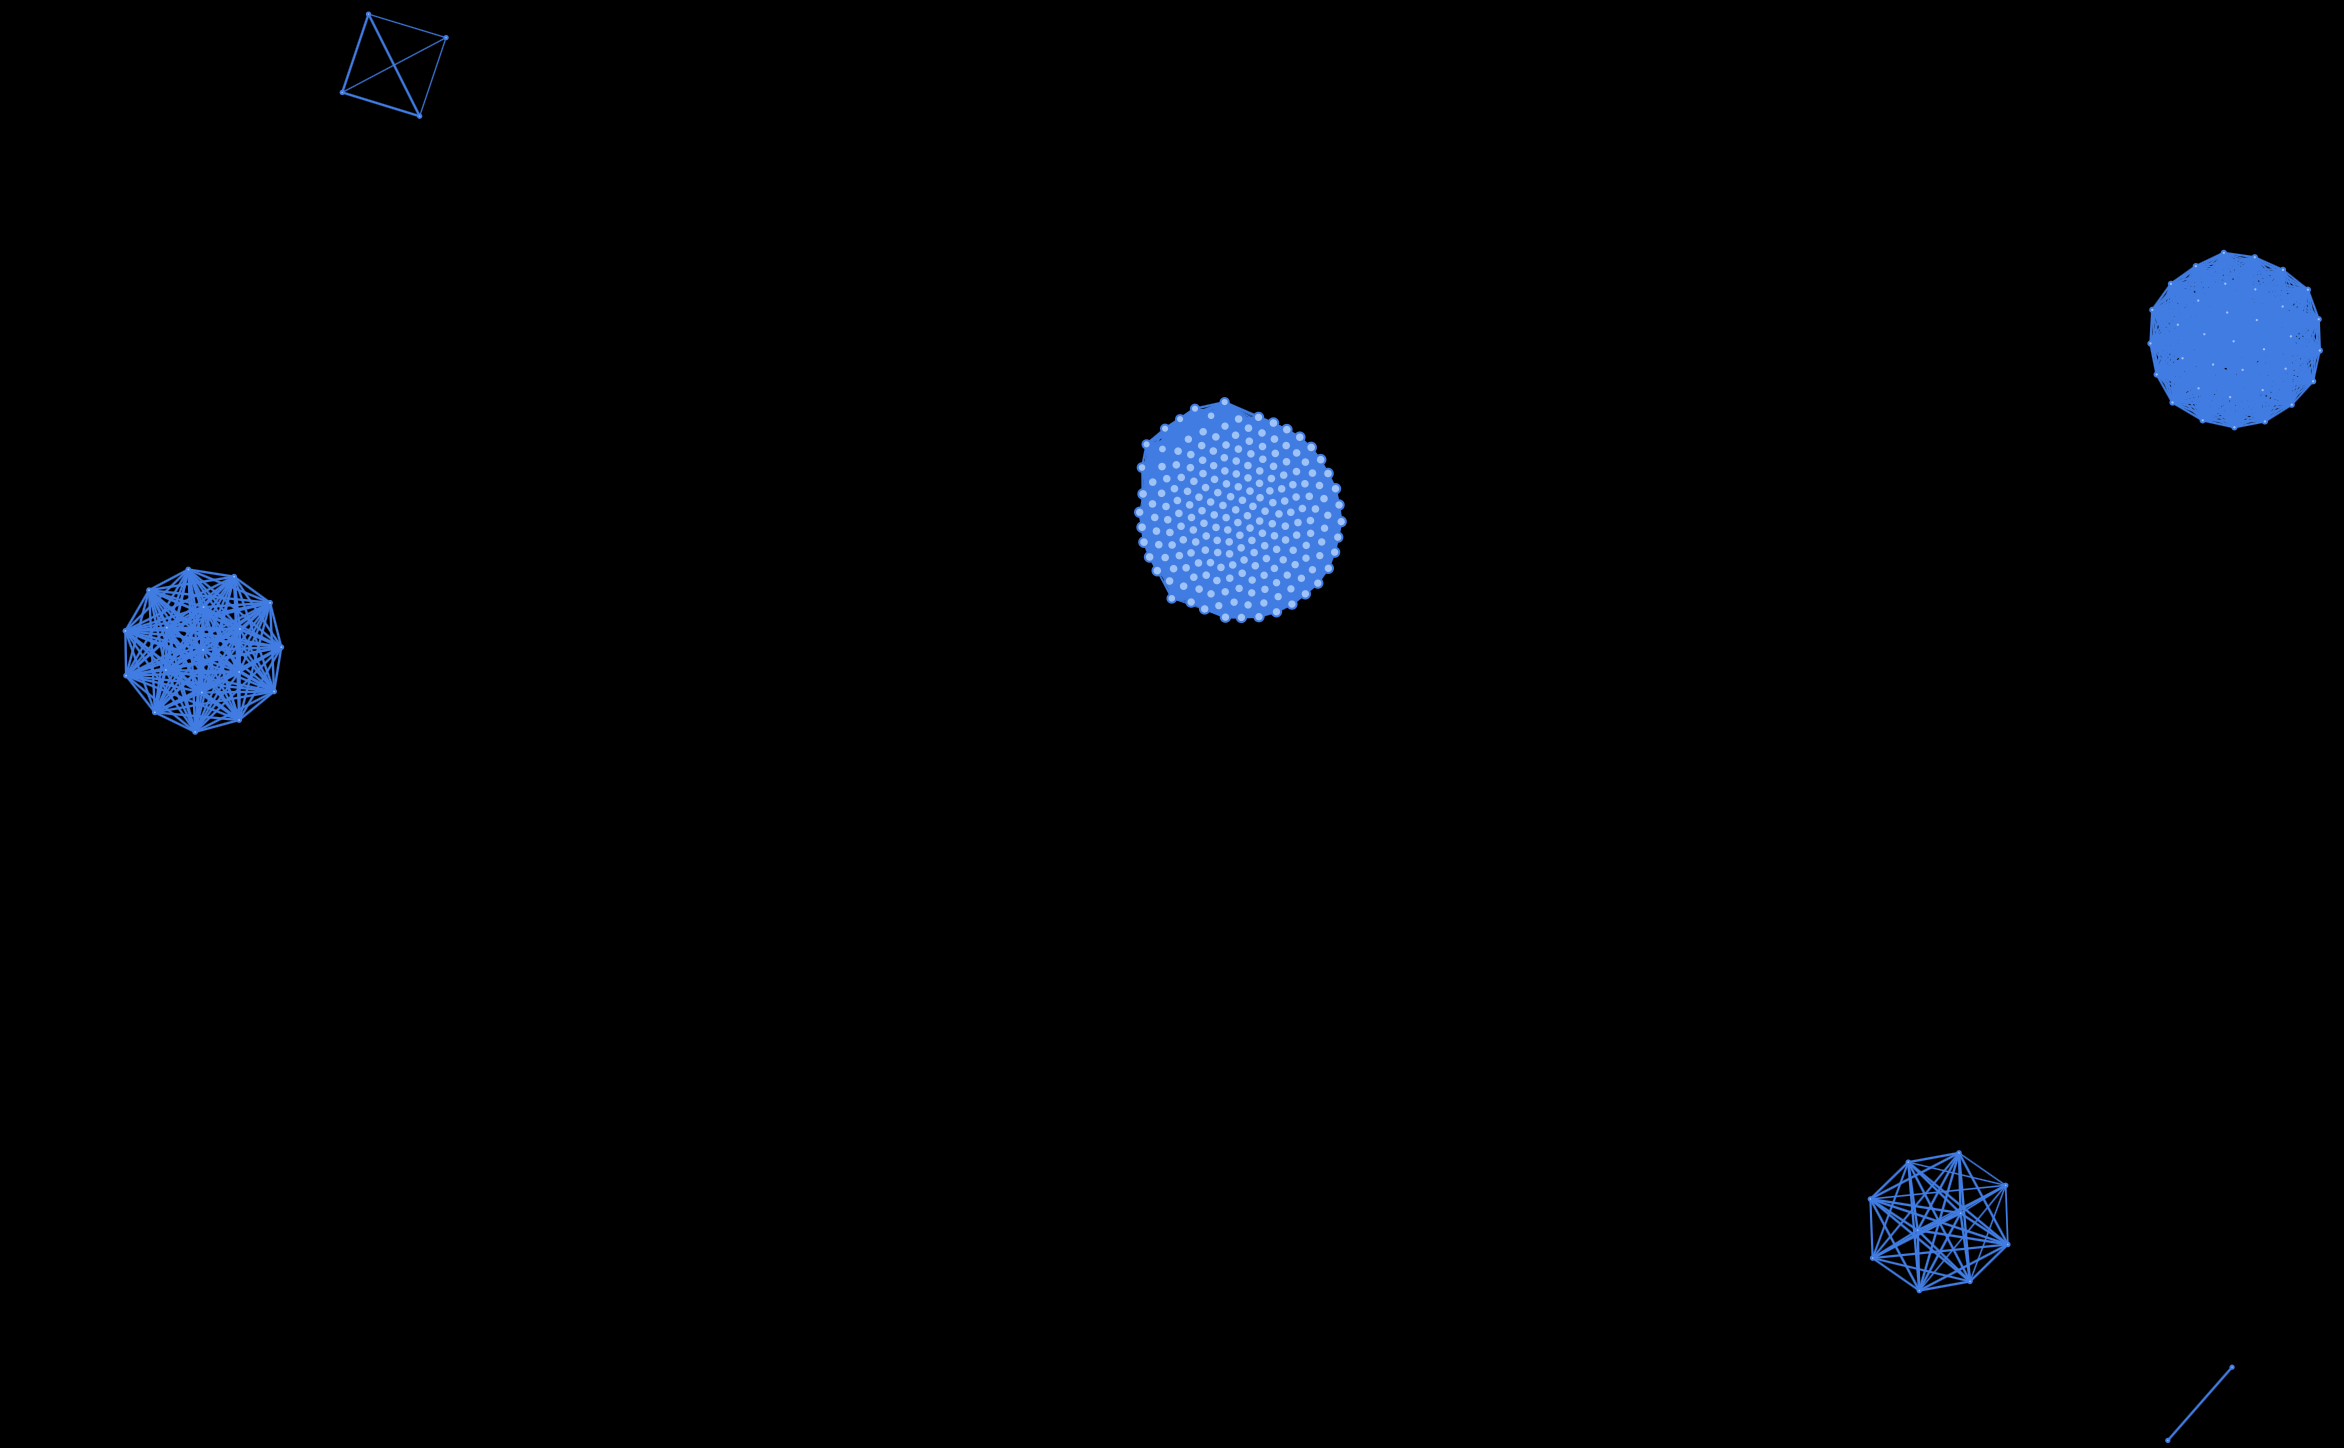
\includegraphics[width=0.6\textwidth]{figures/q2_jointactivities.png}
    \caption{Join-activities network generated through PM4Py}
    \label{fig:figures-q2_jointactivities-png}
\end{figure}

The structure of the obtained network is very different from all networks we have considered up to this point. It consists of six strongly connected components. It seems that all of the components are fully connected, meaning that all resources in a component perform very similar activities. We see that the distinction between components is no longer based on the first letter of the resource name, as we have seen before. The components are now mixtures of these resources. This is not true for one of the components, which only contains A resources.

For the organizational structure this again suggests the supervisor role for the A resources, there are certain activities that are only performed by these resources. Other activities however seem to occur in all of the B, C, D departments. Combining these findings with the findings from the other networks we can assume that the process is structured in such a way that the A department is a supervision department that performs certain specialized tasks. The other departments B, C, D, however perform similar activities (as the join-activity network suggest) but they never mix. This suggests that a case is delegate by the A resources to one of the departments and this department then fully handles the case. It is in a way not a delegation of cases based on certain types of cases, but just a balancing of cases over all departments.

Motivated by these assumptions, we investigated further the data and the relation between the components and the process. We concluded that indeed the components B, C and D perform similar activities: they act on the treatment-related activities. The loose resource is the helicopter, which only acts on the emergency activity. Component A performs the remaining activities: initial trial of the patients, exams, tests, discharge, etc.

\section{Q3. Performance Analysis}
\textlangle Optional: Introduction \textrangle
\paragraph{a)} \textlangle Provide the answer here\textrangle
\paragraph{b)} \textlangle Provide the answer here\textrangle

\section{Q4. Decision Points}

In this section we are interested in the kind of treatment that a patient will undergo based on certain properties. For this we want to create decision trees based on case attributes that can give us deeper insights into which patients receive which treatment.

To do so we are interested in different treatment related events which allow us to group the cases contained in the log according to which kind of treatment they have received. PM4Py offers some functions that can help us create a decision tree that is predicting the end event of a case from the given case and event properties. Since we know that eventually all patients will be discharged from our previous analysis, most of the cases will end in one of the different discharge events (Discharge Init Exam, Discharge Test, Discharge). From this information we cannot infer which treatment was performed before the discharge. Because of this restriction of the raw log, we will preprocess the log before creating decision trees. This preprocessing includes the trimming of all cases. The trace of the case will be trimmed at the point at which a certain event occurs. This event is one of a set of events that describe the treatment of the patient. The events included in this set are \texttt{Treatment A1}, \texttt{Treatment A2}, \texttt{Treatment B}, \texttt{Discharge}, \texttt{Discharge Test} and \texttt{Discharge Init Exam}. These events are either related to a certain kind of treatment, or a discharge. The trace will be cut off at the first of these events that occurs in trace. The discharge events are also included here, for cases that do not receive any treatment. After this preprocessing step, all of the cases end with one of the events specified above.

\paragraph{a)} 
After preprocessing the event log we can now create a decision tree based on it. In the first step of this, we use PM4Py to create the data, targets and classes that will be passed to the sklearn decision tree algorithm. In this step we need to specify which properties of the event log should be used for the decision tree creation. We can specifiy trace based and event based attributes. For our first iteration we included all of the sensible log attributes (for example patient name was removed as it provides no information).

\begin{figure}[h]
    \centering
    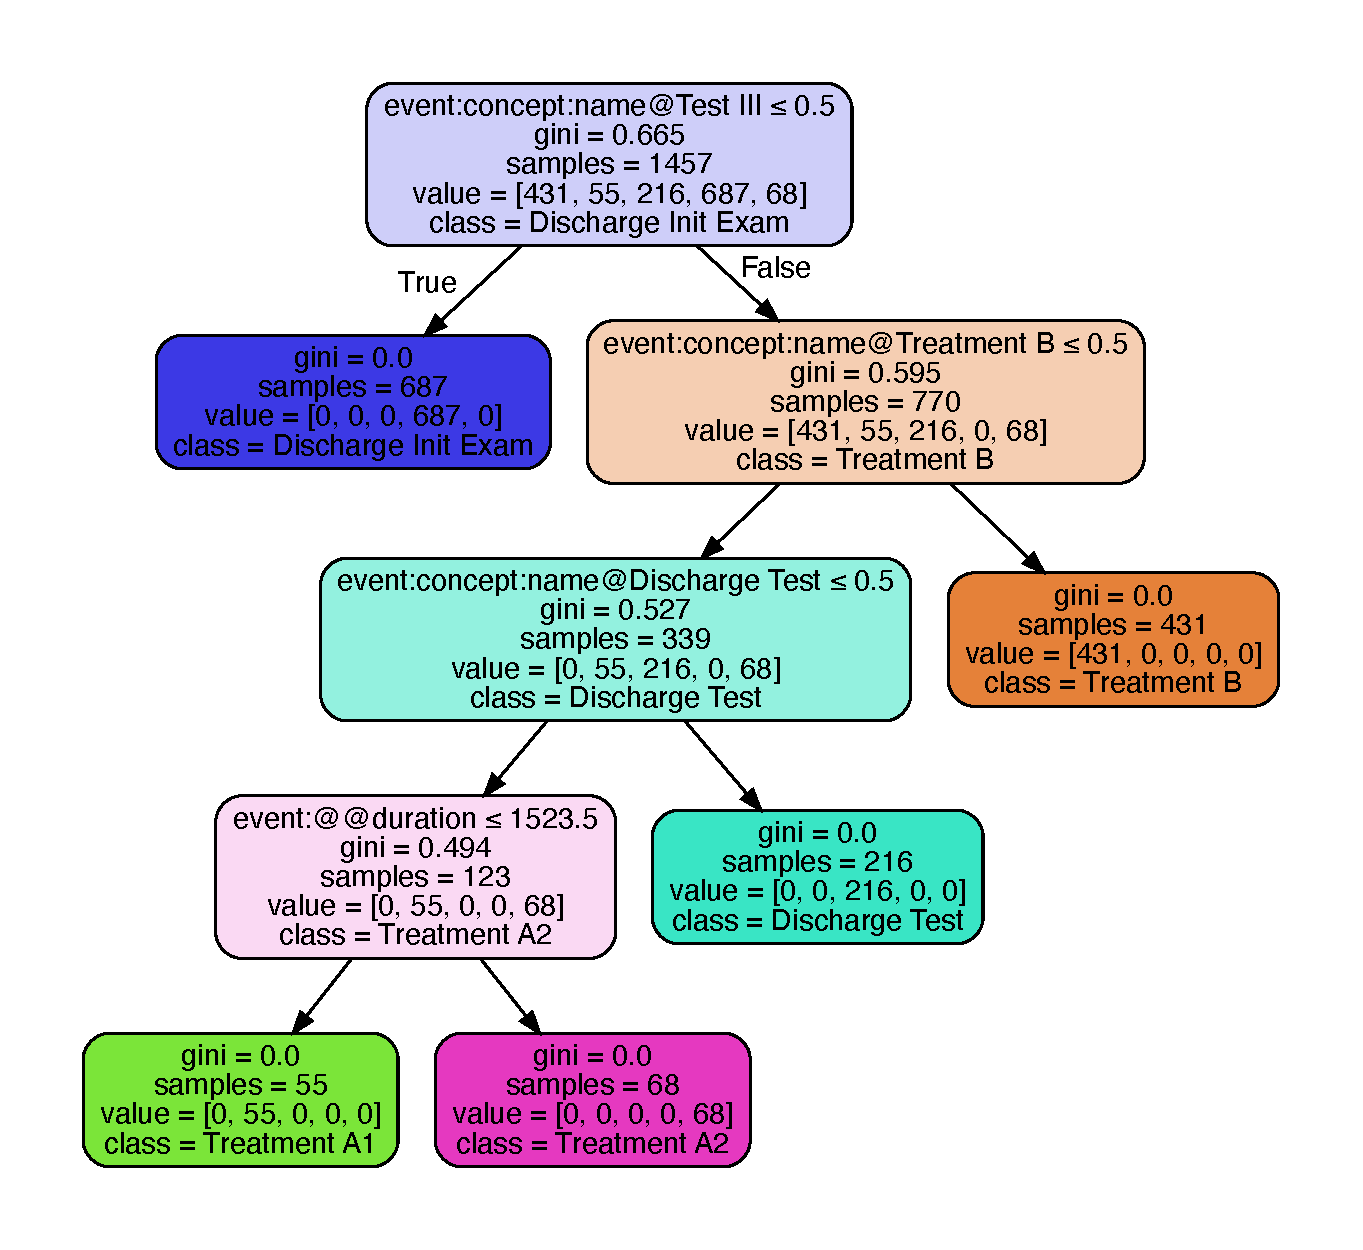
\includegraphics[width=0.5\textwidth]{figures/q4_tree_all.pdf}
    \caption{Decision tree based on all log attributes.}
    \label{fig:figures-q4-tree-all-png}
\end{figure}

The obtained tree can be seen in \ref{fig:figures-q4-tree-all-png}, it is able to perfectly classify all cases, which is unexpected. A closer investigation shows that the tree simply uses the target events themselves to classify the cases, which of course is not wanted. As many of the events are always performed by the same or similar resources, this also holds true for the resource attribute. The two attributes are therefore not suited to be included in a sensible decision tree for this task.
Furthermore we see that the tree once splits using the duration of an event. Since the tree holds no information about which event is related to this duration, we cannot derive meaningful results from this split. The attribute is therefore removed as well. With the remaining age and insurance attributes, we create a new decision tree in the following.

Since the \emph{Discharge Init Exam} event is disproportionally more frequent than all other classes, for this tree we needed to introduce some normalization in order to obtain a sensible tree (Else all nodes would have the same label for a small tree). Additionally, since the tree is not able to perfectly classify all cases anymore, we have to limit the depth and maximum number of child nodes in order to obtain readable results. The depth was capped at 7 and the maximum number of leaf nodes at 8.

\begin{figure}[h]
    \centering
    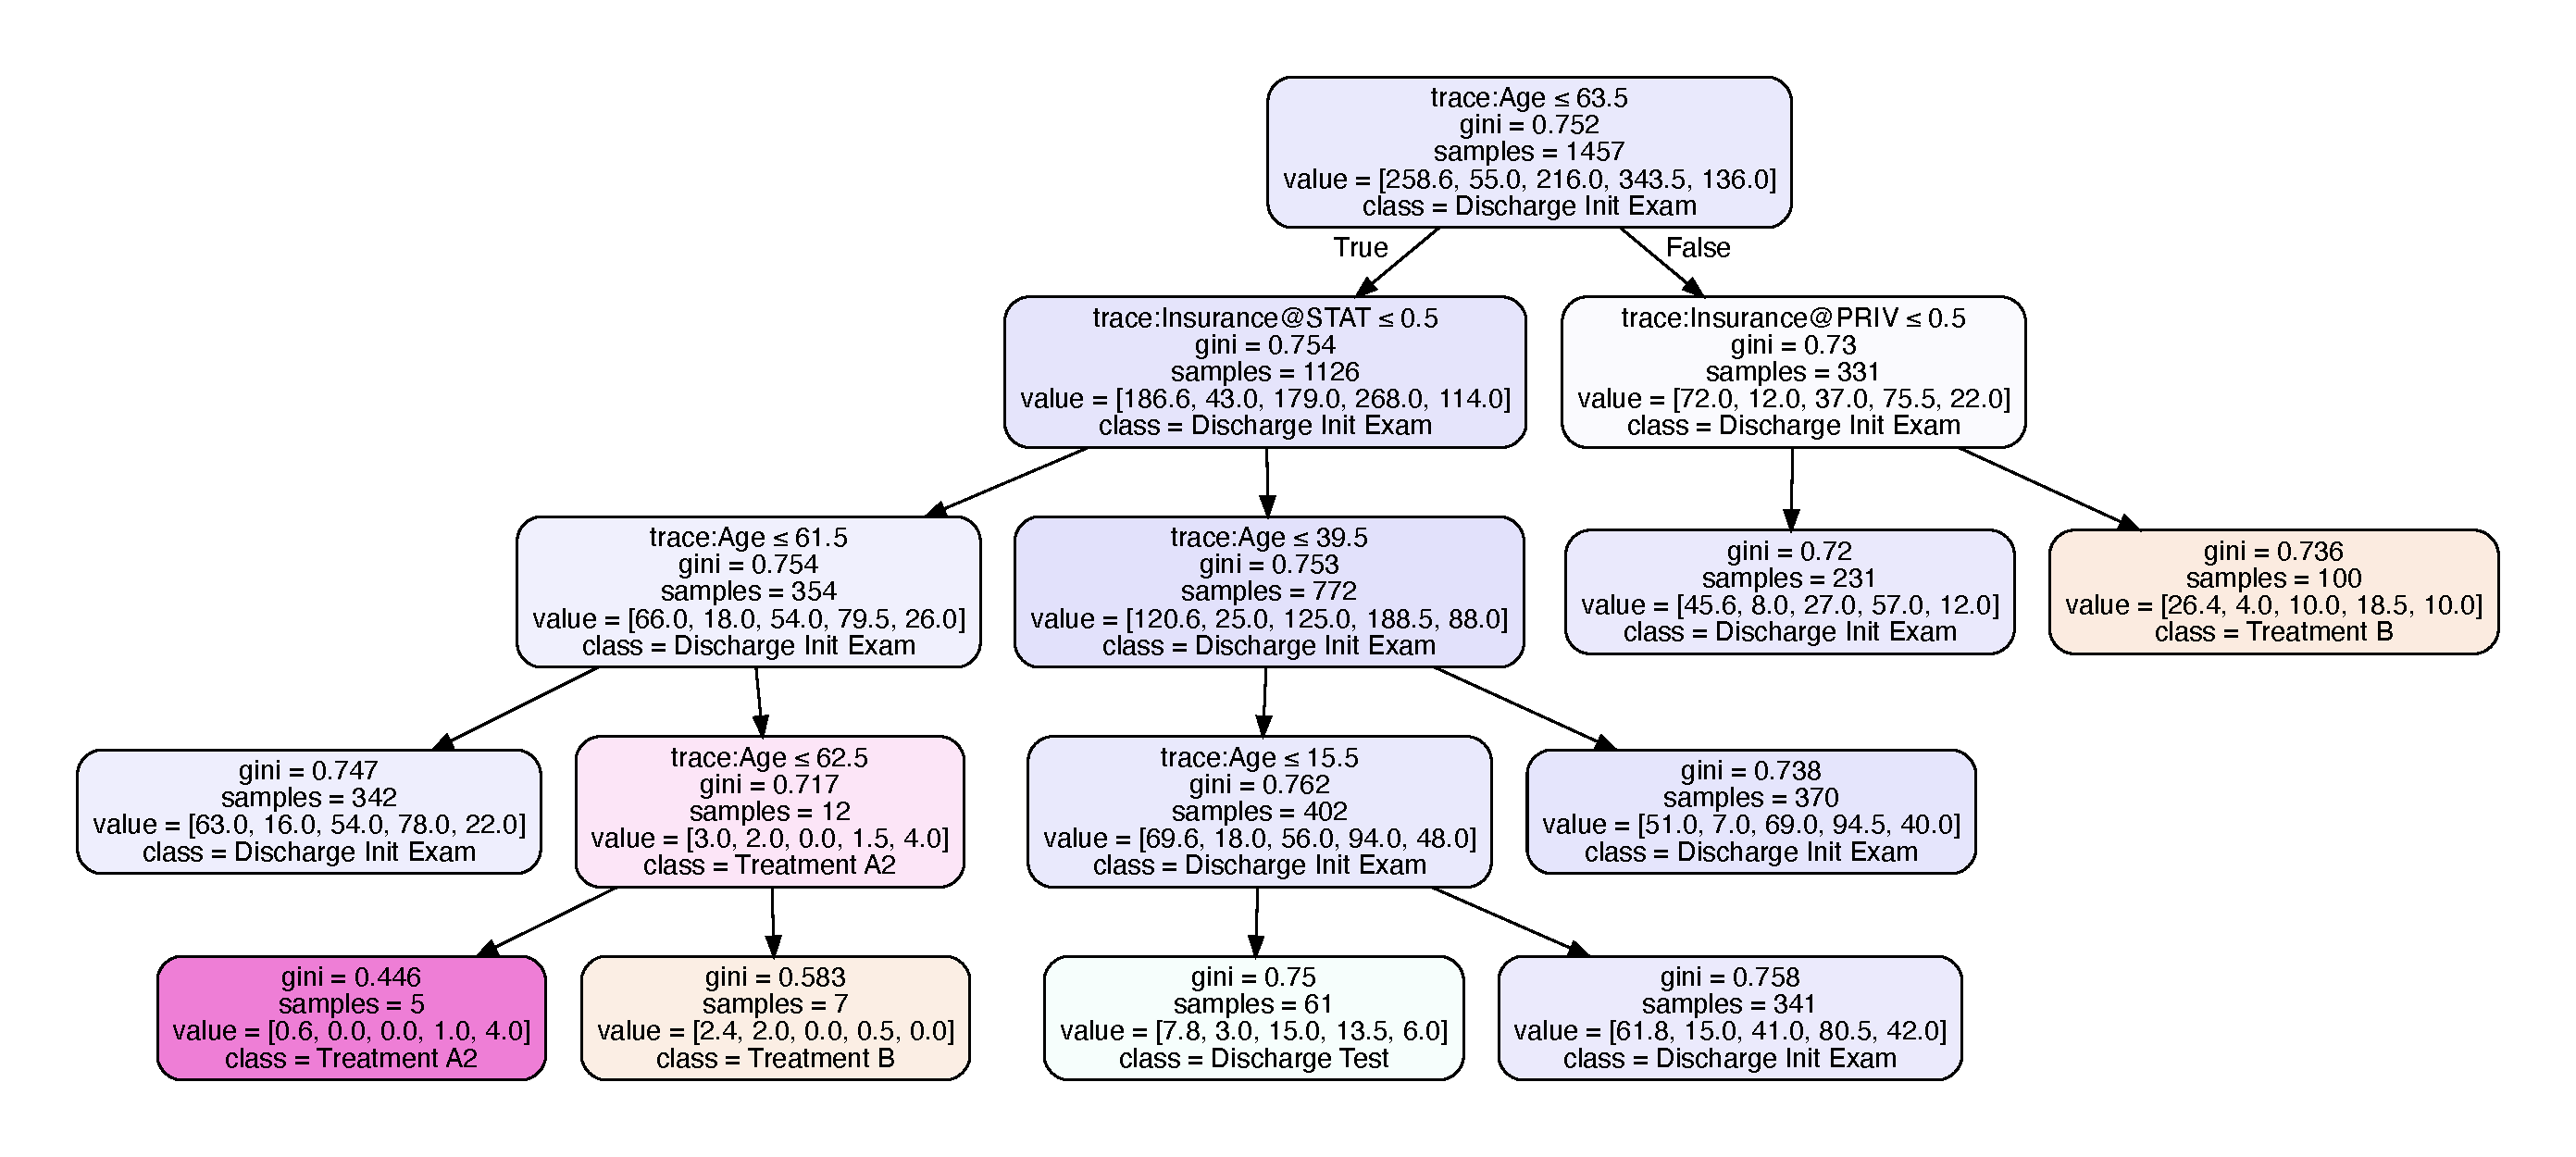
\includegraphics[width=0.9\textwidth]{figures/q4_tree_min.pdf}
    \caption{Decision tree based on the remaining log attributes.}
    \label{fig:figures-q4-tree-min-png}
\end{figure}

The resulting decision tree with a reduced attribute set can be seen in \ref{fig:figures-q4-tree-min-png}, it is much more interpretable. For example we see that patients older than 63.5 years that have a state insurance are more often discharged after the initial exam than ones with a private insurance. This group receives treatment B more frequently.
Furthermore we can observe, that really young patients ($\leq15.5$) are more often discharged after having been tested, while older patients between 15.5 and 39.5 years are more often directly discharged after the initial exam.
In general we can observe that privately insured patients receive any kind of treatment more frequently and are less often discharged without treatment.

\paragraph{b)} 
Based on our analysis in Q2, we know that the resources are heavily related to the facilities. More concrete the first letter of the name of the resource corresponds to the facility of the resource. We will therefore use this property for the distinction between the different facilities.
For this we first create a new property called \emph{facility} that is derived from the first letter of the resource of the event. The unique facilities of the complete log are \texttt{A}, \texttt{B}, \texttt{C}, \texttt{D}, \texttt{I} and \texttt{H}. Based on this we add a new column that documents the move of a patient between two facilities. This is done by shifting the \emph{facility} column down by one. For further implementation details see the documentation. An excerpt of the resulting log can be seen in figure \ref{fig:figures-q4-fac-move-png}.

\begin{figure}[h]
    \centering
    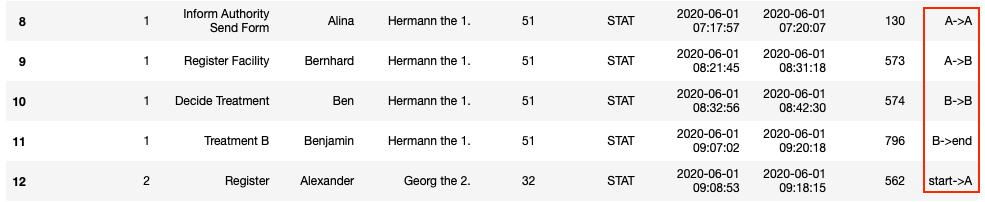
\includegraphics[width=0.9\textwidth]{figures/q4_fac_move.png}
    \caption{The event data after the transformation.}
    \label{fig:figures-q4-fac-move-png}
\end{figure}

Each event now contains the information about the facility move that has happened. For the calculation of these moves the start time of the events is used. That means we assume that the move between facilities happens at the start time of the current event. We can now use this move record to calculate how many patients currently are assigned to a certain facility for every event. We do this by going through the log chronologically and de- or increasing the patient count depending on the facility move that happened. Additionally we have assigned an initial patient count to all of the facilities. This was done because the given dataset is presumably not complete and the facilities have also operated in the time that is not captured by the dataset. A fitting initial value for the facilities was chosen based on the mean value of patients from a previous run of the algorithm and a visual interpretation of the patient counts, of which an excerpt can be seen in \ref{fig:figures-q4-fac-count-png}. We can see that there is some kind of weekly recurring pattern in the patient count of both facilities and that the patient count in facility \texttt{A} steadily rises up until the end.

\begin{figure}[h]
    \centering
    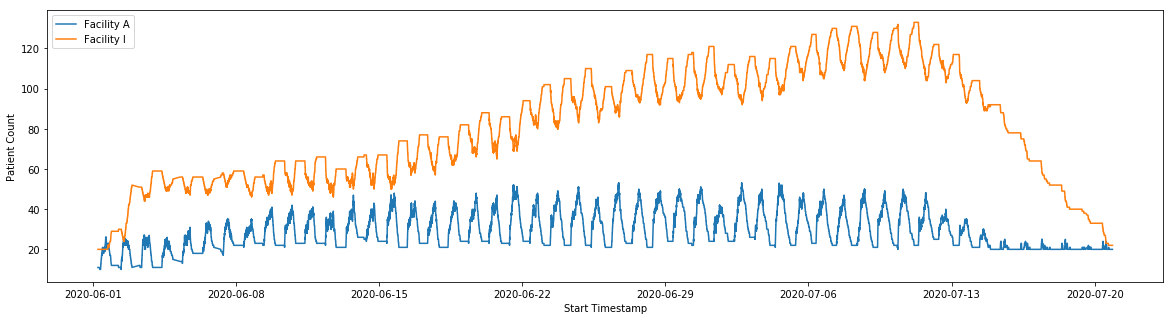
\includegraphics[width=\textwidth]{figures/q4_fac_count.png}
    \caption{The estimated patient count at the facilities \texttt{A} and \texttt{I}.}
    \label{fig:figures-q4-fac-count-png}
\end{figure}

The estimated patient counts at the facilities were joined with the original event log again and transformed into the PM4Py event log representation. Based on that, a decision tree was created as discussed in a). The only attributes that were used were the newly created patient counts. We again applied a normalization and restricted the depth of the tree to 8, while setting the maximum number of leaf nodes to 8. The resulting decision tree can be seen in \ref{fig:figures-q4-facility-tree-png}.

\begin{figure}[h]
    \centering
    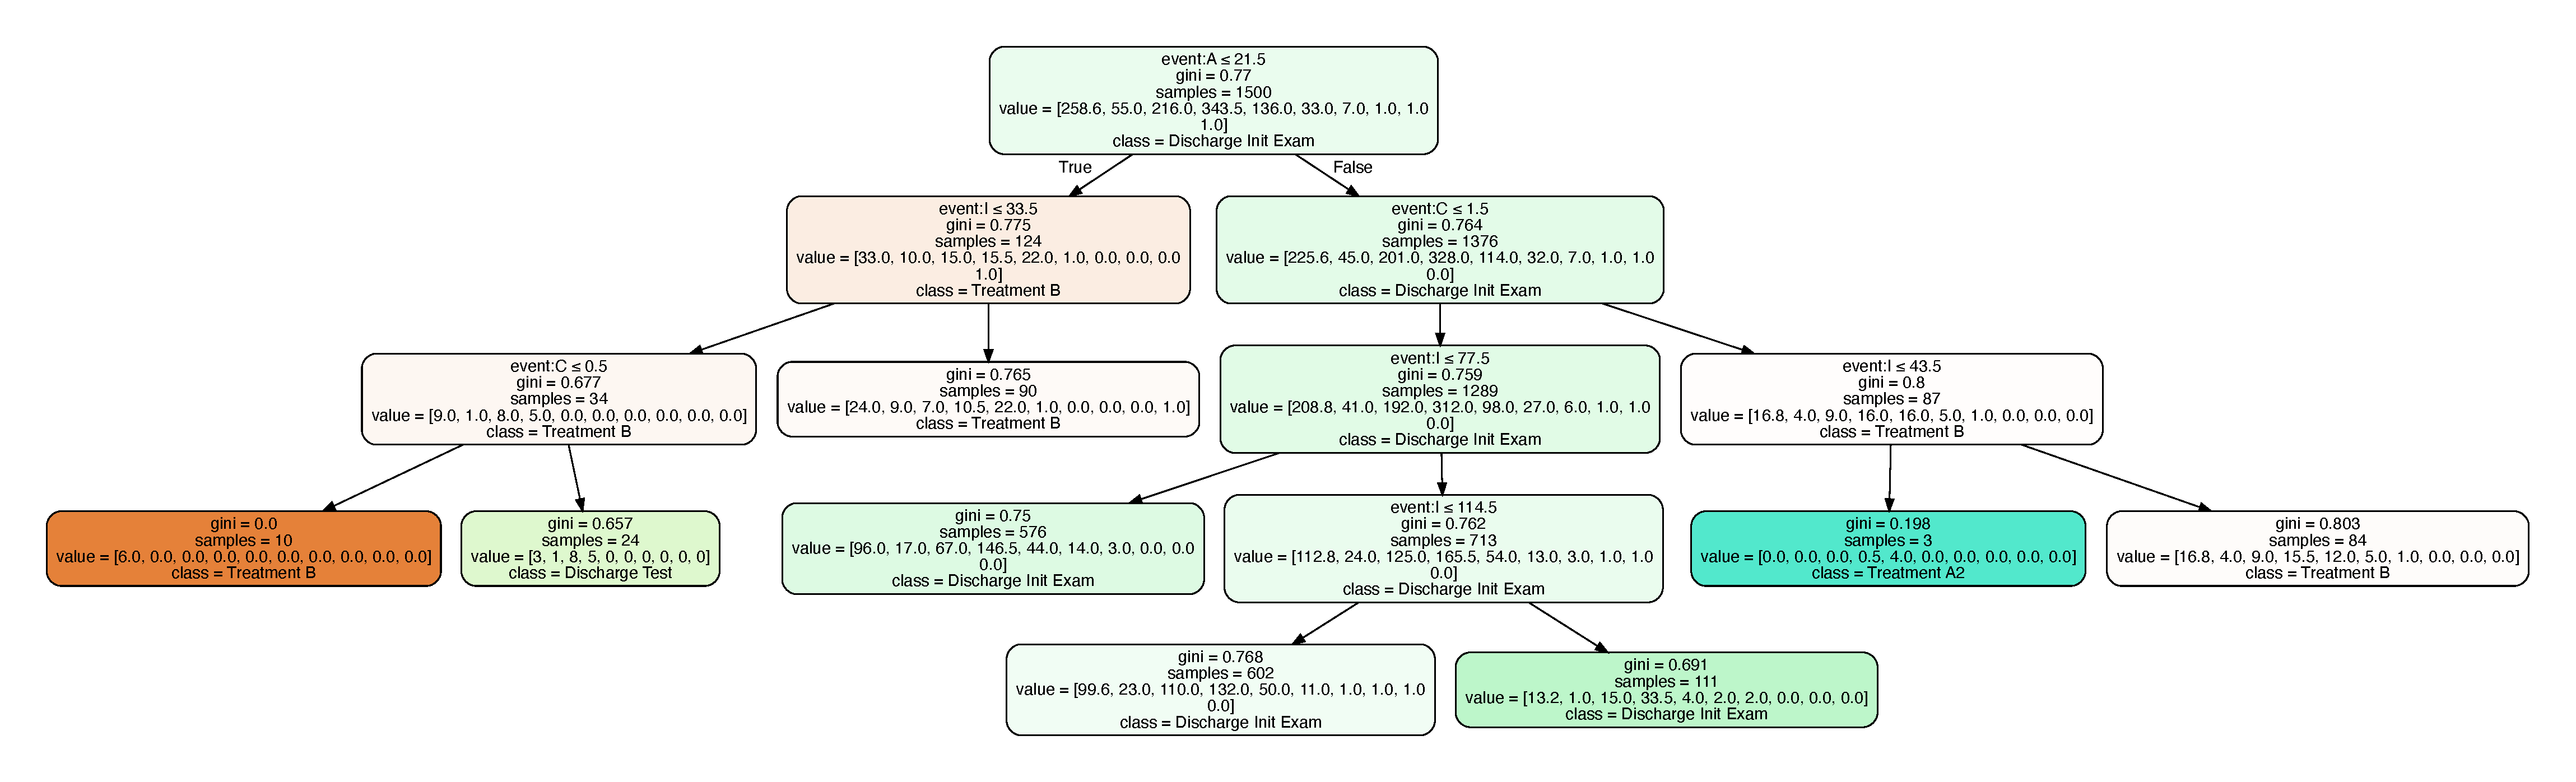
\includegraphics[width=\textwidth]{figures/q4_facility_tree.pdf}
    \caption{The decision tree based on the patient count on the different facilities.}
    \label{fig:figures-q4-facility-tree-png}
\end{figure}

The obtained decision tree is splitting the cases based on the number of patients in each of the facilities. The first split is done on the \texttt{A} facility. We observe that when there are fewer (less than 21) patients in facility \texttt{A}, more treatments are prescribed and less patients are discharged at the initial exam. This could mean that the facility is somehow overloaded when there are many patients, which influences the decision making. 

On the second level we can also observe that there are more initial discharges if there are not many patients in facility \texttt{C}. As discovered in Q2, facility \texttt{C} is mainly concerned with checking treatments, so the reason here might be that when there are more people discharged, there is less need for treatment checks. On the other hand this may also indicate a potential bottleneck in \texttt{C}: There are not enough resources to perform checks, so patients are more frequently discharged.

We also see that the facilities \texttt{B} and \texttt{D} were never used as a splitting criterion, which might indicate that the number of patients in these facilities has no big influence on the treatment and therefore there are enough resources in these facilities.

Facility I is a good indicator for the overall number of "active" patients that are currently in the process, as patients stay in that facility for a longer time (for the control calls). The I facility patient count is therefore also used as a splitting criterion for some nodes. We again observe that treatments are less frequent for higher patient numbers.

In a last step we calculated the number of resources in each facility to compare those numbers with the obtained patient numbers. We see that, although facility \texttt{A} has the highest patient load, it has the lowest number of resources (7) compared to the other "normal" facilities \texttt{B} (18), \texttt{C} (17) and \texttt{D} (17). This is a further indicator that facility \texttt{A} might be understaffed. We also see that there is only one resource in facility \texttt{I}, we have already observed this fact in Q2. This is probably the case as the control calls are somehow automated and performed by a single system, so there can be no resource bottlenecks here.

\section{Q5. Proccess Improve Suggestions}

As was noticed from the very first analysis, the data has some imperfections. This challenged the modeling of the process and limited our analysis. For this, our first suggestion is towards an improvement in the registry of the activities. This could allow for a deeper understanding of the process and increase the possibility of identifying opportunities in it.

When analysing the structure of the resources, we identified the groups of resources that are responsible for the activities. This way it is possible to drive investments towards the resource groups that are more impacting in the problem activities. Unfortunately it is not possible to analyse how is the resources pool impacting the performance of the process, as no sufficient information was provided.

Regarding the performance of the process, the activities with the biggest impact were the control calls. Assuming that these activities are performed while the patients wait for the tests or for the treatments to begin, we can infer that these waiting lines are the most influential factors for the process poor performance. Therefore, we suggest the investment in speeding up the application of the test and the beginning of the treatments.

Still about the performance, we identified that the component C seems to be either underperforming or overloaded, as it is executing longer processes. Thus, further investigation on this group is recommended.

\paragraph{Q4)} 

\newpage
\section{Appendix}

\end{document}

